% !TeX TXS-program:bibliography = txs:///bibtex
% $Id: synbds-noise-synthetic-SJIAOS2015.tex 1784 2016-01-06 14:56:56Z lv39 $
% $URL: https://forge.cornell.edu/svn/repos/lv39_papers/SynLBD/text/SJIAOS2015/synbds-noise-synthetic-SJIAOS2015.tex $

%\documentclass[runningheads,letter,11pt]{llncs}

\documentclass[letter,11pt]{llncs}

\usepackage{amssymb}
\usepackage{amsmath}
\setcounter{tocdepth}{3}
\usepackage{graphicx}
%\usepackage{algorithm}
\usepackage{algpseudocode}
\newenvironment{algorithm}{\begin{center}\hrule\ \\}{\hrule\end{center}}
\usepackage{url}
%\urldef{\mailsa}\path|{joerg.drechsler@iab.de}
%\urldef{\mailsb}\path|{lars.vilhuber@cornell.edu}
%\urldef{\mailsc}\path|erika.siebert-cole, peter.strasser, lncs}@springer.com|
\newcommand{\keywords}[1]{\par\addvspace\baselineskip
\noindent\keywordname\enspace\ignorespaces#1}
\usepackage{csvsimple}
\usepackage{tikz}
\usepackage{calc}
\usepackage[printonlyused]{acronym}
\usepackage{listings}

% for math cal
\usepackage[cal=euler]{mathalfa}

%\usepackage{comment}
\usepackage{etoolbox}

%%%%%%% The "final" flag toggles the final version of the proposal. When set
%%%%%%% to true, all comments are hidden, the page is set to the correct size,
%%%%%%% and any `fix' information is drawn normally.
\newtoggle{final}
%\toggletrue{final}
\togglefalse{final}
%%%%%%%%%%%%%%%%%


\iftoggle{final}{
	\usepackage[disable]{todonotes}
    }{
    \usepackage[textsize=scriptsize]{todonotes}
    }

% todo-enabled version: \margincomment{}{} command to put comments about text into the 
%margin.
\newcommand{\margincomment}[2]{% % 1=initials, 2=comment
\todo[size=\footnotesize]{\textbf{\uppercase{#1}:}~#2}
}

%TCIDATA{Version=5.00.0.2570}
%TCIDATA{LaTeXparent=0,0,sw-edit.tex}

% $Id: acrodefs.tex 1692 2015-07-15 20:04:17Z lv39 $
% $URL: https://forge.cornell.edu/svn/repos/lv39_papers/SynLBD/text/JSM2015/acrodefs.tex $
%
% Define acronyms to be used in the text here. See
% http://www.mackichan.com/index.html?techtalk/456.htm~mainFrame for usage in
% Scientific workplace context


\acrodef{ACS}{American Community Survey} 
\acrodef{AHEAD}{Study of Assets and Health Dynamics Amongst the Oldest Old}
\acrodef{ASCII}{American Standard Code for Information  Interchange} %, typically used to 
%denote raw text files in PC or Unix environments
\acrodef{ASM}{Annual Survey of Manufacturers}
\acrodef{BDS}{Business Dynamics Statistics}
\acrodef{BED}{Business Employment Dynamics}
\acrodef{BES}{Business Expenditure Survey}
\acrodef{BLS}{Bureau of Labor Statistics}
\acrodef{BRB}{Business Register Bridge}
\acrodef{BR}{Business Register}
\acrodef{CAC}{Cornell Center for Advanced Computing}
\acrodef{CBP}{County Business Patterns}
\acrodef{CBSA}{Core-Based Statistical Area}
\acrodef{CER}{Covered Earnings Records}
\acrodef{CES}{Center for Economic Studies}
\acrodef{CEW}{Covered Employment and Wages}%. Employment statistics program run by BLS 
%in  conjunction with all states, also known as ES-202. Generally, when used  in this document, 
%refers to public-use tabulations from the CEW, as  opposed to the confidential microdata 
%received directly from the states.
\acrodef{CISER}{Cornell Institute for Social and Economic Research}
\acrodef{CIT}{Cornell Information Technologies}
\acrodef{CODA}{Children of Depression}
\acrodef{CPI}{Consumer Price Index}
\acrodef{CPI-U}{Consumer Price Index (All Urban Consumers)}
\acrodef{CPR}{Composite Person Record}
\acrodef{CPS}{Current Population Survey}
\acrodef{CRADC}{Cornell Restricted Access Data Center}
\acrodef{CTC}{Cornell Theory Center}
\acrodef{DCC}{Data Confidentiality Committee}
\acrodef{err}{excess reallocation rate}
\acrodef{jcr}{job creation rate}
\acrodef{jdr}{job destruction rate}
\acrodef{jrr}{job reallocation rate}
\acrodef{wrr}{worker reallocation rate}
\acrodef{DER}{Detailed Earnings Record}
\acrodef{DRB}{Disclosure Review Board}
\acrodef{DWS}{Displaced Worker Supplement}
\acrodef{ECF}{Employer Characteristics  File}
\acrodef{EHF}{Employment History Files}
\acrodef{EIN}{Employer Identification Number}
\acrodef{ERR}{Excess Reallocation Rate}
\acrodef{FHFA}{Federal Housing Finance Agency}
\acrodef{FIPS}{Federal information processing standards codes}
\acrodef{FTI}{Federal Tax Information}
\acrodef{GAL}{Geocoded Address List}
\acrodef{GIS}{Geographic Information System}
\acrodef{HPI}{House Price Index}
\acrodef{HRS}{Health and Retirement Study}
\acrodef{ICF}{Individual Characteristics File}
\acrodef{IRB}{Institutional Review Board}
\acrodef{IRS}{Internal Revenue Service}
\acrodef{ISR}{Institute for Social Research}
\acrodef{JCR}{Job Creation Rate}
\acrodef{JDR}{Job Destruction Rate}
\acrodef{JOLTS}{Job Openings and Labor Turnover Survey}
\acrodef{JRR}{Job Reallocation Rate}
\acrodef{LAUS}{Local Area Unemployment Statistics}
\acrodef{LBD}{Longitudinal Business Database}
\acrodef{LDB}{\ac{BLS}'s Longitudinal Business Database}
\acrodef{LED}{Local Employment Dynamics}
\acrodef{LEHD}{Longitudinal Employer-Household Dynamics}
\acrodef{LMI}{Labor Market Information}
\acrodef{LODES}{LEHD Origin-Destination Employment Statistics}
\acrodef{MBR}{Master Beneficiary Record}
\acrodef{MEF}{Master Earnings File}
\acrodef{MER}{Master Earnings Record}
\acrodef{MLS}{Mass Layoff Statistics}
\acrodef{MMS}{Methodology, Measurement, and Statistics}
\acrodef{MN}{Minnesota}
\acrodef{MSA}{Metropolitan Statistical Area}
\acrodef{MSD}{Metropolitan Statistical Division}
\acrodef{MWR}{Multiple Worksite Report}
\acrodef{NAICS}{North American Industry Coding System}
\acrodef{NECTA}{New England  City and Town Area}
\acrodef{NIA}{National Institute on Aging}
\acrodef{NIST}{National Institute of Standards and Technology}
\acrodef{NLSY}{National Longitudinal Study of Youth}
\acrodef{NSF}{National Science Foundation}
\acrodef{NSTA}{NAICS SIC Treatment of Auxiliaries}
\acrodef{OTM}{OnTheMap}
\acrodef{PCF}{Person Characteristics File}
\acrodef{PHF}{Person History File}
\acrodef{PIK}{Protected Identity Key}
\acrodef{PSID}{Panel Study of Income Dynamics}
\acrodef{QCEW}{Quarterly Census of Employment and Wages}
\acrodef{QWI}{Quarterly Workforce Indicators}
\acrodef{RDA}{Restricted Data Application}
\acrodef{RDC}{Research Data Center}
\acrodef{RUN}{Reporting unit number}
\acrodef{SEIN}{State employer identification number}
\acrodef{SEINUNIT}{SEIN reporting unit}
\acrodef{SEPB}{Summary of Earnings and Projected Benefits} % confidential 
%SSA                                % file
\acrodef{SESA-ID}{State Employment Security Agency ID}
\acrodef{SESA}{State Employment Security Agency}
\acrodef{SIC}{Standard Industry Classification}
\acrodef{SIPP}{Survey of Income and Program Participation}
\acrodef{SLID}{Survey of Labour and Income Dynamics}
\acrodef{SPF}{Successor-Predecessor File}
\acrodef{SRMI}{Sequential Regression Multiple Imputation}
\acrodef{SSA}{Social Security Administration}
\acrodef{SSI}{Supplemental Security Income}
\acrodef{SSN}{Social Security Number}
\acrodef{SSR}{Supplemental Security Record}
\acrodef{SynLBD}{Synthetic \ac{LBD}}
\acrodef{U2W}{Unit-to-Worker Impute}
\acrodef{UI}{Unemployment Insurance}
\acrodef{WB}{War Babies}
\acrodef{WIA}{Workforce Investment Act}
\acrodef{WIB}{Workforce Investment Board}
\acrodef{WRR}{Worker Reallocation Rate}
\acrodef{WTS}{Windows Terminal Services}

% Usage in the later text:
%  \ac{acronym}         Expand and identify the acronym the first time; use
%                       only the acronym thereafter 
%  \acf{acronym}        Use the full name of the acronym.
%  \acs{acronym}        Use the acronym, even before the first corresponding
%                       \ac command 
%  \acl{acronym}        Expand the acronym without using the acronym itself.

%%% Local Variables: 
%%% mode: latex
%%% TeX-master: "proposal"
%%% End: 



\newcommand{\mytitle}{Using partially synthetic microdata to protect sensitive cells in business 
statistics}
\newcommand{\myshorttitle}{Partially Synthetic BDS}
\newcommand{\myversion}{\today}  %alternate version

\newcommand{\alert}{}
\newcommand{\sep}{,}

\begin{document}

\mainmatter  % start of an individual contribution

% first the title is needed
\title{\mytitle}

% a short form should be given in case it is too long for the running head
\titlerunning{\myshorttitle}

% the name(s) of the author(s) follow(s) next
%
% NB: Chinese authors should write their first names(s) in front of
% their surnames. This ensures that the names appear correctly in
% the running heads and the author index.
%
\author{Javier Miranda \and Lars Vilhuber \thanks{\textbf{Miranda:} U.S. Bureau of the Census, Washington, DC, USA \email{javier.miranda@census.gov}. \textbf{Vilhuber:} (Corresponding Author) Cornell University, Ithaca, NY, USA, \email{lars.vilhuber@cornell.edu}}}
%
%\authorrunning{J. Miranda and L. Vilhuber}
% (feature abused for this document to repeat the title also on left hand pages)

% the affiliations are given next; don't give your e-mail address
% unless you accept that it will be published
%\institute{U.S. Bureau of the Census, Washington, DC, USA \email{javier.miranda@census.gov} \and
%Cornell University, Ithaca, NY, USA, \email{lars.vilhuber@cornell.edu}, Corresponding author\\
%}
\institute{}
%
% NB: a more complex sample for affiliations and the mapping to the
% corresponding authors can be found in the file "llncs.dem"
% (search for the string "\mainmatter" where a contribution starts).
% "llncs.dem" accompanies the document class "llncs.cls".
%

%\toctitle{Lecture Notes in Computer Science}
%\tocauthor{Javier Miranda and Lars Vilhuber}
\maketitle

%\begin{center}
%{\large Preliminary - Do not cite without permission from the authors.}
%This version: \today
%\end{center}

%\date{\myversion}
\begin{abstract}
% $Id: abstract.tex 1659 2015-02-01 00:33:21Z lv39 $
% $URL: https://forge.cornell.edu/svn/repos/lv39_papers/SynLBD/text/JSM2015/abstract.tex $
We describe and analyze a method that blends records from both observed and synthetic 
microdata into public-use tabulations on establishment statistics. The resulting tables use 
synthetic data only in potentially sensitive cells. We describe different algorithms, and present 
preliminary results when applied to the Census Bureau's Business Dynamics Statistics and 
Synthetic Longitudinal Business Database, highlighting accuracy and protection afforded by the 
method when compared to existing public-use tabulations (with suppressions). 
\keywords{synthetic data, statistical disclosure limitation, time-series, local labor markets, gross 
job flows, confidentiality protection}
\end{abstract}

\clearpage
\section{Introduction}
\label{sec:intro}
% $Id: intro.tex 1773 2015-12-18 22:07:18Z lv39 $ 
% $URL: https://forge.cornell.edu/svn/repos/lv39_papers/SynLBD/text/SJIAOS2015/intro.tex $

Statistics based on detailed business data are increasingly relied upon to make informed 
decisions by firms and governments. Novel statistics, for instance on business startups and firm 
dynamics \cite{BDS2}, are valuable additions to the toolbox of evidence-based policy and 
business decisions. At the same time, the sparsity and skewness of business data makes 
disclosure avoidance a challenge. Early \ac{CBP} statistics (before the advent of noise infusion as 
a disclosure avoidance measure) had between 10 and 40 percent of values suppressed.\footnote{Example taken from 2004 CBP, national by NAICS tabulations, across all size and NAICS cells.} 

In recent years, the use of fully or partially synthetic data has allowed the publication of 
increasingly detailed statistics. Going back to the seminal contributions of \cite{rubin93} and 
\cite{little93}, the release of statistics based on partially synthetic data in the U.S. Census 
Bureau's \ac{LODES} \cite{Ashwin2008} and \ac{ACS} 
\cite{Rodriguez2007,hawala2008,zayatzjsm2009}⁠ strikes a 
new 
balance between detailed statistics and appropriate disclosure avoidance. Other cases of using 
synthetic data for the purpose of tabulation exist
\cite{AbowdEtAl2012,RePEc:cen:wpaper:13-19}.
  Furthermore, partially 
synthetic microdata \cite{Drechsler2012,KinneyEtAl2011,ssafinal} has been released to 
end-users as a access and analysis mechanism \cite{CES-WP-2014-10}.

In this paper, we explore the use of tabulations based on partially synthetic data as a disclosure 
avoidance mechanism for certain at-risk tabulation cells. This is similar in spirit to the originally 
proposed uses of synthetic data \cite{little93,rubin93}, and follows similar uses of  
partially synthetic data in the \ac{ACS} \cite{hawala2008,zayatzjsm2009}⁠. Our approach differs in 
that we address longitudinal consistency of the data explicitly, an important feature of the 
statistics underlying our paper. 

To illustrate and implement the proposed mechanism, we use the \acf{BDS}. The \ac{BDS} were 
first released in 
2008, providing novel statistics on business startups on a comprehensive basis for the U.S. 
economy \cite{BDS2}. They have been used in a number of recent publications, addressing %\margincomment{Re MHS}{Addressed Martha's comment here.}
questions of  job creation and destruction, establishment births and deaths, and firm startups and shutdowns %\margincomment{LV}{Added additional references}
\cite{NBERw16300,RePEc:bin:bpeajo:v:43:y:2011:i:2011-02:p:73-142,10.1257/jep.28.3.3,pugsley2014grown}. 
The \ac{BDS} are sourced from confidential microdata in the \acf{LBD}. It
provides measures of business openings and closings, and job creation and destruction, by a variety of cross-classifications (firm and establishment age and size, industrial sector, and geography).
Since the first release, additional cross-tabulations have been added each year: initially provided 
only based on  firm charateristics, tabulations based on establishment characteristics were later 
added, as were additional geography cross-tabulations (Metropolitan Statistical Area, and 
Metro/Non-Metro).  Sensitive data are currently protected through suppression. However, as 
additional tabulations are being developed, at ever more detailed geographic levels, the number 
of suppressions increases dramatically.\footnote{The next set of expansions include plans to 
provide additional industry and geography detail.}  

We leverage the existence of a sophisticated partially synthetic data file the Synthetic LBD 
\cite{SynLBD20,KinneyEtAl2011}, 
henceforth \acs{SynLBD} -- in combination with the techniques first expressed in 
\cite{Gittings2009thesis} and \cite{RePEc:bes:jnlasa:v:105:i:492:y:2010:p:1347-1357} to replace 
sensitive cells with tabulations based on synthetic 
data.  A previous paper \cite{psd2014a} described early results from the implementation of the 
simplest algorithm described here. In this version, we refine those algorithms, and present new 
results. 
We start by describing the extent of suppressions in the \ac{BDS}, then lay out the algorithm to 
combine synthetic and confidential data for the purposes of tabulation. Preliminary results are 
discussed, and an outlook given on the next steps necessary to achieve a robust public-use 
tabulation. 



%\section{The dynamically-consistent multiplicative noise infusion model\label{sec:disclosure:fuzz}}
%\label{sec:disclosure-proofing}
%\label{sec:confidentiality}
%\input{disclosure-proofing}
 
\section{Current Protection Methods}
\label{sec:item_suppression}
% $Id: item-suppression.tex 1784 2016-01-06 14:56:56Z lv39 $ 
% $URL: https://forge.cornell.edu/svn/repos/lv39_papers/SynLBD/text/SJIAOS2015/item-suppression.tex $

BDS processing uses primary and secondary suppressions, derived from a \emph{P} percent rule, as disclosure avoidance mechanism. All cells of a potential publication table are analyzed to make sure no identifying information about a particular business, household, or individual  is released to the public. In the case of the BDS, cells where the top 2 firms account for more than \emph{P} percent of the total value of the cell are flagged for suppression. The precise \emph{P} value is not disclosed to minimize the possibility of reidentification by potential attackers. Secondary suppressions are identified so as to minimize the amount of information loss in a given table row or column. To this end, the search algorithm looks for candidate cells that contain the least amount of employment, and suppresses their content. Protecting these secondary cells might require a third round of supressions given the presence of column totals in the tables.
Once the tables are analyzed and the necessary cells suppressed, each table row that contains a 
suppression is flagged, and the modified table released to the public.\footnote{Note that in 
some data 
release formats (SAS) individual suppressed cells are not separately flagged, only the row that 
contains at least one suppressed cell.}  A necessary feature of this disclosure mechanism is that 
a 
large number of  secondary suppressions  are necessitated by the need to protect the cell that is 
the primary disclosing cell. The public-use data, of course, doesn't allow the identification of 
which suppressions are primary or secondary suppressions.


Table~\ref{tab:bds_e} describes the extent to which suppressions occur in the  published 
establishment-level \ac{BDS} \cite{BDS2012} (Table~\ref{tab:bds_f} in 
the appendix also describes the similar pattern in firm-level statistics). The number of cells in 
each table is indicated, as are the percent of cells with  suppression of some variable ({\tt 
d\_flag=1}),  and the percent of cells where ``Job Creation by Entrants''  or ``Job Creation by 
Continuers'' is suppressed. 
%\margincomment{LV}{Added mention of JC continuers, and table additional column here.}
Other  variables, also present on the establishment-level \ac{BDS}, are never suppressed. 

% created in SynBDS/programs/01*sas sequence

%\csvautotabular{programs/bds_e_suppressions_multi.csv}
%\begin{table}
%\caption{Suppressions in establishment-level BDS\label{tab:bds_e}}
%\centering
%\begin{tabular}{|lc|r|rr|}\hline%
%               &                 &\bfseries Number &\multicolumn{2}{c|}{\bfseries Suppressions (\%)}\\
%\cline{4-5}
%\bfseries Type & \bfseries Level &\bfseries of     &                            & \bfseries Job creation\\
%                            &                              &\bfseries  cells& \bfseries Any  &\bfseries by entrants\\
%\hline
%\csvreader[head to column names,late after line=\\,late after last line=\\\hline]%
%{programs/bds_e_suppressions_multi.csv}{}%
%{\typename & \level & \cells & \percentsup  & \jcbirths}%
%\multicolumn{5}{p{0.6\textwidth}}{\footnotesize Note: Cells are year $x$ categories, where the 
%number of categories varies by published table.}
%\end{tabular}
%\end{table}


%\begin{table}
%\caption{Suppressions in establishment-level BDS\label{tab:bds_e}}
%\centering
%\begin{tabular}{|l|r|rrr|}\hline%
%               &                 \bfseries Number &\multicolumn{3}{c|}{\bfseries Suppressions (\%)}\\
%\cline{3-5}
%\bfseries Type  &\bfseries of     &                            & \multicolumn{2}{c|}{\bfseries Job creation}\\
%\cline{4-5}
%                                                          &\bfseries  cells& \bfseries Any  &\bfseries by entrants &\bfseries 
%                                                          by continuers\\
%\hline
%\csvreader[head to column names,late after line=\\,late after last line=\\\hline]%
%{programs/bds_e_suppressions_multi.csv}{}%
%{\typename &  \cells & \percentsup  & \jcbirths &\jcconts}%
%\multicolumn{4}{p{0.6\textwidth}}{\footnotesize Note: Cells are year $x$ categories, where the 
%number of categories varies by published table.}
%\end{tabular}
%\end{table}

Clearly, while the usefulness of the data to users would seem to increase for more detailed 
cross-tabulations, that same detail, under current disclosure avoidance rules, leads to increased 
suppression, and thus less effective data utility. Suppression is worse for some variables than 
for others. Establishment and firm counts are never suppressed following County Business 
Patterns and Disclosure Review Board rules. By contrast job creation and 
destruction, and establishment birth and deaths may be suppressed. 



%\section{Combining Synthetic and Protected Data}
\section{Alternative Protection Methods}
\label{sec:synthetic_method}
% $Id: synthetic.tex 1784 2016-01-06 14:56:56Z lv39 $
% $URL: https://forge.cornell.edu/svn/repos/lv39_papers/SynLBD/text/SJIAOS2015/synthetic.tex $

%\margincomment{LV}{Added this paragraph}
In this section, we describe a protection system which uses tabulations from synthetic data, in a variety of implementations, to compensate for the suppressions generated by the current protection system. They should be considered extensions or complements to the current protection methods, since we describe and implement them within the constraints of the current system. In particular, our definition of sensitive cells is driven entirely by the current protection system. For comparison purposes, we also (partially) implement an  alternate protection system, multiplicative noise infusion. 

\subsection{Synthetic Data Tabulations}


The \ac{SynLBD} \cite{SynLBD20} is a synthetic dataset on establishments with proven analytic 
validity along several critical dimensions \cite{KinneyEtAl2011}. Additional improvements are 
currently being developed \cite{KinneyEtAl2013,CES-WP-2014-12}. A growing number of 
researchers have used the \ac{SynLBD}, and their continued use contributes to the 
improvement of the \ac{SynLBD}. 

The use of the \ac{SynLBD} for the purposes outlined in this paper is particularly appealing, 
because its analytic validity has been independently established, while maintaining a high level 
of data privacy. Based on the variables already available on the released \ac{SynLBD}, tabulations that 
use the \ac{SynLBD} as an input presumably require no additional disclosure avoidance review. %\margincomment{re MHS}{This was already addressed.}
Only tabulations involving state and sub-state geography should require 
additional review since geographic variables were removed from the disclosure request that 
approved the  release to the public of the SynLBD.%
\footnote{The Census Disclosure Review Board has not pronounced itself on the disclosure 
avoidance methodology proposed here as of December 2015.}
 
The available \ac{SynLBD} is released as a single implicate, and by design, may distort an analysis by a potentially large an amount. The use of additional implicates for the purposes of BDS table creation may be desirable and will be assessed in later work. 

%\margincomment{Lars}{Needs to be rewritten}
In this paper, we propose and evaluate several algorithms that complement the existing 
\ac{BDS} disclosure avoidance methodology (primary and secondary suppression, PSS). In all 
cases, we allow the PSS methodology to determine which cells are sensitive. Once identified, 
sensitive cells as well as some additional cells are modified using tabulations based on synthetic 
establishments.  

The first algorithm, which we will call the ``drop-in algorithm'', simply replaces a cell that has 
been suppressed with its synthetic-data equivalent, i.e., the equivalent table cell from a 
tabulation based on the \ac{SynLBD} alone. The second algorithm, called 
``forward-longitudinal algorithm'', is slightly more complicated. At any point in time $t$, if a 
(expanded) suppression algorithm identifies a cell that \emph{would} be suppressed under 
PSS, all 
establishments that contribute to that cell in  time period $t$ are replaced by synthetic 
establishments that match on certain characteristics $Z$ in periods $t-p$ through $t$, for $t$ 
and the next $n$ periods. Synthetic and observed values are then tabulated to create the 
release statistics. To smooth the phasing out of the synthetic establishments, we define weights 
$w(n)$ that decline monotonically from unity to zero for synthetic establishments, and increase 
correspondingly for real establishments. 
If $Z$ 
describes only the margin characteristics for the table in question 
(denoted by $k$ below), and not any additional characteristics, and for $p=n=0$, the algorithm 
is similar to the ``drop-in'' algorithm, but creates consistent higher-level tables automatically. 
On the other hand, the ``forward-longitudinal algorithm'' cannot be done post-publication 
without the re-release of historical tabulations.

In this paper, we will restrict ourselves to $p=0$ and $n=\lbrace 0,4 \rbrace$ in order to assess the 
time-consistency of the proposed algorithms for a single implicate.
%\margincomment{Re MHS}{This had already been addressed.}
We have 
previously assessed the impact of Algorithm 1 (defined below)  \cite{psd2014a}.
Assessing the impact of using multiple implicates as well as identifying 
acceptable values of $Z$, $p$, and $n$ is deferred to  future work.

\subsection{Definitions}
The variable of interest is establishment employment $e_{jt}$, with establishments indexed by 
$j$ and years indexed by $t$. All other variables (job creation and destruction from 
establishment entry, exit, expansion and contraction) are derived from that basis. For instance, 
an establishment is ``born'' at time $t$ if employment is positive for the first time in $t$:
\begin{eqnarray}
\label{eq:e_birth}
birth_{jt} &=& \left \lbrace 
\begin{array}{rl}
1 &\mbox{if}~~  e_{jt} > 0 ~~ \mbox{and}  ~~e_{jt-s} = 0 ~~\forall s\geq 1~~\\
0 &\mbox{otherwise}
\end{array} \right .
\end{eqnarray}
We will denote aggregations using capital letters, so (national) employment is denoted as
%\margincomment{Re MHS}{Corrected confusing switch in notation.}
\begin{equation}
\label{eq:national_e}
E_{\cdot t} = \sum_{j=1}^J e_{jt}
\end{equation}
and (national) births are
\begin{equation}
\label{eq:national_birth}
Birth_{\cdot t} = \sum_{j=1}^J birth_{jt}.
\end{equation}
An establishment $j$ has a vector of  time-invariant and time-varying
characteristics $k_t(j)$, such as industry and geographic location (time-invariant), but also 
derived 
characteristics, such as establishment or firm age and size. In a slight abuse of notation, $j \in 
K_t^\prime$ describes the set of firms at time $t$ such that $k_t(j)=k^\prime$.   Generically, 
\begin{equation}
\label{eq:sum_X}
X_{k^\prime t} =  \sum_{j \in K_t^\prime} x_{jt}
\end{equation}
describes the different aggregations across establishments having characteristics $k^\prime$ at 
time $t$, for instance aggregations by establishment age or metropolitan areas, referred to as 
``confidential BDS'' (\textbf{BDS$^{conf}$}).
%

For any establishment $j$, the synthesized version of variable $x_{jt}$ (from a single implicate) is 
denoted $\tilde{x}_jt$. The vector $\tilde{k}_t(j)$ describes the set of characteristics when using 
the synthetic dataset, which will generally differ from $k_t(j)$ because time-varying derived 
characteristics such as age and size will differ (at this time, neither industry nor geography are 
synthesized). We designate the set of  establishments $j$ with synthetic characteristics 
$\tilde{k}_t(j)$ as $\tilde{K}_t^\prime$, and will refer to them as  ``synthetic 
establishments.''  Aggregations across synthetic establishments are
\begin{equation}
\label{eq:sum_X_synth}
\tilde{X}_{k^\prime t} =  \sum_{j \in \tilde{K}_t^\prime} \tilde{x}_{jt}
\end{equation}
and will be referred to as ``synthetic BDS'' (\textbf{BDS$^{(s)}$}).

Finally, suppression rules for (aggregate) variable $X$ are captured by $I_{t}^X$, such that the 
releasable variable $X^o$  under the current regime (PSS) can be described by

%\begin{equation}
%\label{eq:supp_x}
%X_{k^\prime t}^o = X_{k^\prime t}  I_{t}^X 
%\end{equation}
\begin{eqnarray}
\label{eq:supp_x}
X_{k^\prime t}^o &=& \left \lbrace 
\begin{array}{rl}
X_{k^\prime t} &\mbox{if}~~  I_{kt}^X = 1 \\
\mbox{missing} &\mbox{otherwise}
\end{array} \right .
\end{eqnarray}

For later 
reference, we denote the tabulations created as per (\ref{eq:supp_x}) as \textbf{BDS$^{(0)}$}.
%We will denote by $K_t^\prime \subset K$ the subset of the domain of $K$, such as certain industries, or age categories within certain geographic areas, so that $J_t^j \in K_t^\prime$ 

\subsection{Algorithm 1: Drop-in}

We can now express the ``drop-in'' algorithm, leading to the released variable $X^{(i)}$, as:
\begin{algorithm}
%\caption{(n=0) Drop-in}
\label{alg1n}
\begin{algorithmic}
\If {$I_{t}^X = 0$ }
        \State {$X_{k^\prime t}^{(i)} =\tilde{X}_{k^\prime t} $}
\Else
    \State {$X_{k^\prime t}^{(i)} = X_{k^\prime t} $}
\EndIf
\end{algorithmic}
\end{algorithm}

Thus, simply computing a ``SynBDS'', based on the \ac{SynLBD}, in parallel to the computation 
of the \ac{BDS}, based on the confidential \ac{LBD}, and replacing suppressed cells with their 
fully synthetic counterparts, yields a dataset without missing cells. Note that we have assumed 
the existence of only one synthetic implicate; the use of multiple synthetic implicates would 
replace the second component of Algorithm~1 with  
$X_{k^\prime t}^{(i)} = \frac{1}{\ell} \sum_{l=1}^{\ell} \tilde{X}_{k^\prime t l} $, the average across 
$\ell$ 
implicates. In 
general, increasing the number of implicates will improve the analytic validity, but reduce the 
protection provided by the synthesis process. 

Because no time-consistency is imposed, this method can lead to seam biases or higher 
intertemporal variance. Furthermore, only interior cells are adjusted, but no margins are 
corrected, likely leading to discrepancies in the global table structure. Raking would solve that 
issue, but is not explored here. %We will return to this issue in Section~\ref{sec:analysis}. 

%\margincomment{LV}{Additional paragraph for the smoothed drop-in}
In order to smooth the time-series generated by this process, and to provide a comparison to 
the microdata-based smoothing outlined later in this section, we generalize the above algorithm 
to combine not just synthetic tabulations in periods with suppression, but also in later periods. 
Thus, in periods that follow a period with $I_{t}^X = 1$, we average synthetic tabulations with 
non-suppressed tabulations, for up to $n$ periods:
%\addtocounter{algorithm}{-1}
%\newpage
\begin{algorithm}
%\caption{Weighted Drop-in}
{\bf Algorithm 1: Weighted Drop-in}
\hrule
\label{alg1}
\begin{algorithmic}
\State {$s^* = min_{s \in [0,n]} $ s.t. $I_{t-s}^X = 0$ }
\If { $n>0$ and $\exists s^*$ }
    \State {$X_{k^\prime t}^{(i)} =  \frac{s^*}{n} X_{k^\prime t}  
               + \left (1-\frac{s^*}{n} \right ) \tilde{X}_{k^\prime t} $}
\ElsIf { $n=0$ and $I_{t}^X = 0$}
    \State {$X_{k^\prime t}^{(i)} =  \tilde{X}_{k^\prime t} $}
\Else
        \State {$X_{k^\prime t}^{(i)} ={X}_{k^\prime t} $}               
\EndIf
\end{algorithmic}
\end{algorithm}

For $n=0$ this reduces to the prior expression. 
For later 
reference, we denote the tabulations created by Algorithm~1 as \textbf{BDS$^{(i)}$} 
in its general form, and as \textbf{BDS$^{(in)}$}  when $n=0$.
%\margincomment{Re MHS}{I hesitated, because when using $^{2}$ it might be confused for "squared", whereas $^{ii}$ is not ambiguous}

\subsection{Algorithm 2: Forward-longitudinal}

In part to address the possible time-inconsistencies we propose an 
alternative algorithm.  In order to minimize future seam issues, we downweight or remove 
establishments (or 
firms) that 
contribute to sensitive cells of tabulations with characteristics $k^\prime t$, for $t$ and the next 
$n-1$ periods. These establishments are (partially) replaced by  synthetic establishments that 
match on 
characteristics $k^\prime t$, and we simply replace the observed values in the database $x_{js}$ 
with the synthetic values $\tilde{x}_{js}$ (for all variables), for $s=t,\dots,t+n$.  %
%
For convenience, 
denote by $J_{k^\prime t}^-$ the set of establishments that are to be excluded from tabulations at time $t$, and $J_{k^\prime t}^+$ the set of synthetic establishments that are added to the 
tabulations as replacements. We construct $J_{k^\prime t}^-$ by first adding establishment identifiers that meet the suppression conditions $I^X_{kt}$ at time $t$. In addition, we assign establishments to 
$J_{k^\prime s}^-$ for the $n$ periods after a cell stops being sensitive as well. Formally, we  add 
those same establishments to ``future''  $I^X_{ks}$, for $s \in [t+1,t+n]$ if $n>0$. Thus, at any 
point in time $t$, the set $J_{k^\prime t}^-$ contains establishments that met suppression 
conditions now and in the past, i.e.,   in $[t-n,t]$.   
%\margincomment{Re MHS}{Moved the sentence here, clarified (hopefully) language.}
%
In order to ``smooth'' the tabulated data, we specify  a 
per-establishment weight $w_{js} \in [0,1]$, applied to the observed data, that increases from 
$0$ in $t$ to $1$ in $t+n$, 
and  a per-establishment weight $\tilde{w}_{js}$, applied to the synthetic data, that decreases 
from $1$ in $t$ to $0$ in 
$t+n$, thus ``blending in''  the real establishments, and ``blending out'' the synthetic 
establishments. Setting $w_{js} = 0, s \in [t,t+n-1]$ and $\tilde{w}_{js}=1, s \in [t,t+n-1]$ effectively 
removes the real establishments from the tabulation, being completely  replaced by the synthetic 
establishments.
%
In its simplest 
form, the algorithm can be expressed as

%\addtocounter{algorithm}{1}
\begin{algorithm}
%\caption{Forward-longitudinal}
{\bf Algorithm 2: Forward-longitudinal}
\hrule
\label{algorithm:2}
\begin{algorithmic}
\State {Compute: $X_{k^\prime t} = \sum_{j \in K_t^\prime} x_{jt}$}
\State{Compute: $I_{t}^X$}
\If {$I_{t}^X = 0$  }
   \State {// Suppression condition met for cell $k^\prime$}
    \State {Assign all $j \in K_t^\prime$ to $J_{k^\prime s}^-$ for $t \leq s \leq t+n$}
    \State {Assign all $j \in \tilde{K}_t^\prime$ to $J_{k^\prime t}^+$ for $t \leq s \leq t+n$}
\EndIf
\State { Compute: %
$$
X_{k^\prime t}^{(iiw)} = 
               \sum_{j \in \left \lbrace K_t^\prime \cap J_{k^\prime t}^+ \right \rbrace }
                               \tilde{w}_{jt} \tilde{x}_{jt} 
	          +
	          \sum_{j \in  K_t^\prime \wedge j \in J_{k^\prime t}^-  }
	                                  w_{jt}  {x}_{jt} 
	          +
	          \sum_{j \in  K_t^\prime \wedge j \notin J_{k^\prime t}^-  }
	                                         {x}_{jt} 
$$}

\end{algorithmic}
\end{algorithm}
%
where the first component is the (possibly down-weighted) sum of synthetic data, the second 
component is the (up-weighted) sum of observed establishments in periods after they are no 
longer part of sensitive cells, and the third component is sum of establishments that were not 
part of sensitive establishments in the past (or outside of the window $[t-n,t]$). 

For $n=\infty$, $J_{t}^-$ is an absorbing set, which seems undesirable. For $n=0$, this is similar 
to, 
but not equal to Algorithm~1. Note that in contrast to Algorithm~1, all higher level tabulations 
are consistent, since the replacement occurs at the microdata level, not at the tabulation cell 
level.

Consider the case for period $s$ for which $I_{s}^X=1$ and $I_{s-1}^X=0$, i.e., the suppression 
conditions no longer apply. By assignment in period $s-1$, some LBD establishments are still 
assigned to $J_{k^\prime s}^-$, and some synthetic establishments are still part of $ J_{k^\prime 
t}^+$. However, new LBD establishments that are identified by $k^\prime$ are counted in 
$X_{k^\prime t}^{(ii)}$ by virtue of the second sum. Equivalently, establishments (synthetic or 
real) that move out of $k^\prime$ (because they age or grow out of the category) naturally drop 
out of $X_{k^\prime t}^{(ii)}$. Note that because we condition on $J_{k^\prime}$, synthetic 
establishments that naturally exit tabulation cell $k^\prime$ are not counted toward an 
alternative tabulation cell $k^\star$, unless that cell is \textit{also} a candidate for suppression. 
For reference, we denote the tabulations created by Algorithm~2 as \textbf{BDS$^{(ii)}$}.


\subsection{Multiplicative Noise Infusion}
%\margincomment{LV}{This entire section added}
Multiplicative noise infusion was originally proposed by \cite{EvansZayatzSlanta1998}. Implementations include the \ac{QWI} \cite{AbowdEtAl2009} and the \ac{CBP}. We apply multiplicative noise to employment counts and payroll measures (although our analysis in this paper only focuses on employment-based measures). 

Multiplicative noise is drawn  for each establishment $j$ 
from a bilateral ramp distribution:%
\begin{equation}\arraycolsep=1.4pt\def\arraystretch{2.2}
	p\left( {\delta _{j}}\right) =\left\{ {{%
			\begin{array}{ccl} 
			\dfrac{ {1+ b - \delta } }{\left( {b - a} \right)^2}
					&,&\;\delta \in \mbox{ }\left[ {1+a,1+b} \right] \\ 
				\dfrac{ {\delta - (1 - b)} }{\left( {b - a} \right)^2} 
				&,&\;\delta \in \left[ {1 - b,1 - a} \right] \\ 
				0&,&\;\mbox{ otherwise } \\
				 \end{array}%
		}}\right. 
	\end{equation}%
%	\begin{equation}
%		F\left( {\delta _{j}}\right) =\left\{ {{%
%				\begin{array}{*{20}c} {\mbox{0},\;\delta < {2-b} } \\ {{\left[ {\left( {\delta + b - 2} \right)^2} \right]} \mathord{\left/ {\vphantom {{\left[ {\left( {\delta + b - 2} \right)^2} \right]} {\left[ {2\left( {b - a} \right)^2} \right]}}} \right. \kern-\nulldelimiterspace} {\left[ {2\left( {b - a} \right)^2} \right]},\;\delta \in \left[ {2 - b,2 - a} \right]\mbox{ }} \\ {\mbox{0.5}, \;\delta \in \mbox{ }\left( {2-a,a} \right)\mbox{ }} \\ {\mbox{0.5} + {\left[ {\left( {b - a} \right)^2 - \left( {b - \delta } \right)^2} \right]} \mathord{\left/ {\vphantom {{\left[ {\left( {b - a} \right)^2 - \left( {b - \delta } \right)^2} \right]} {\left[ {2\left( {b - a} \right)^2} \right]}}} \right. \kern-\nulldelimiterspace} {\left[ {2\left( {b - a} \right)^2} \right]},\;\delta \in \mbox{ }\left[ {a,b} \right]\mbox{ 
%						}} \\ {\mbox{1}, \;\delta > {b} } \\ \end{array}}}\right. 
%		\end{equation}%
		
\noindent where $a={c}/{100}$ and $b={d}/{100}$ are constants chosen
		such that the true value is distorted by a minimum of $c$ percent and a
		maximum of $d$ percent. This produces a random noise factor centered around 1 with
		distortion of at least $c$ and at most $d$ percent. Figure~\ref%
		{fig:fuzzgraph} depicts such a distribution.  The noise factor is drawn only once,  and 		retained for all time periods after the initial assignment. For this exercise, we set $c=10$ and $d=25$ percent as plausible numbers, for illustration only. Note that these numbers are in general confidential, and we have no knowledge of the actual parameters used in \ac{QWI} and \ac{CBP}. Both \ac{QWI} and  \ac{CBP} use  slightly more complex noise infusion algorithms that takes into account the firm structure and table structure, and include suppression for the smallest cells where multiplicative noise provides insufficient protection. None of those additional features are implemented here.
%
We denote the tabulations protected by noise infusion as \textbf{BDS$^{(n)}$}.
		
		
%\begin{figure}
%	\centering
%	\caption{Empirical distribution of noise\label{fig:fuzzgraph}}
%	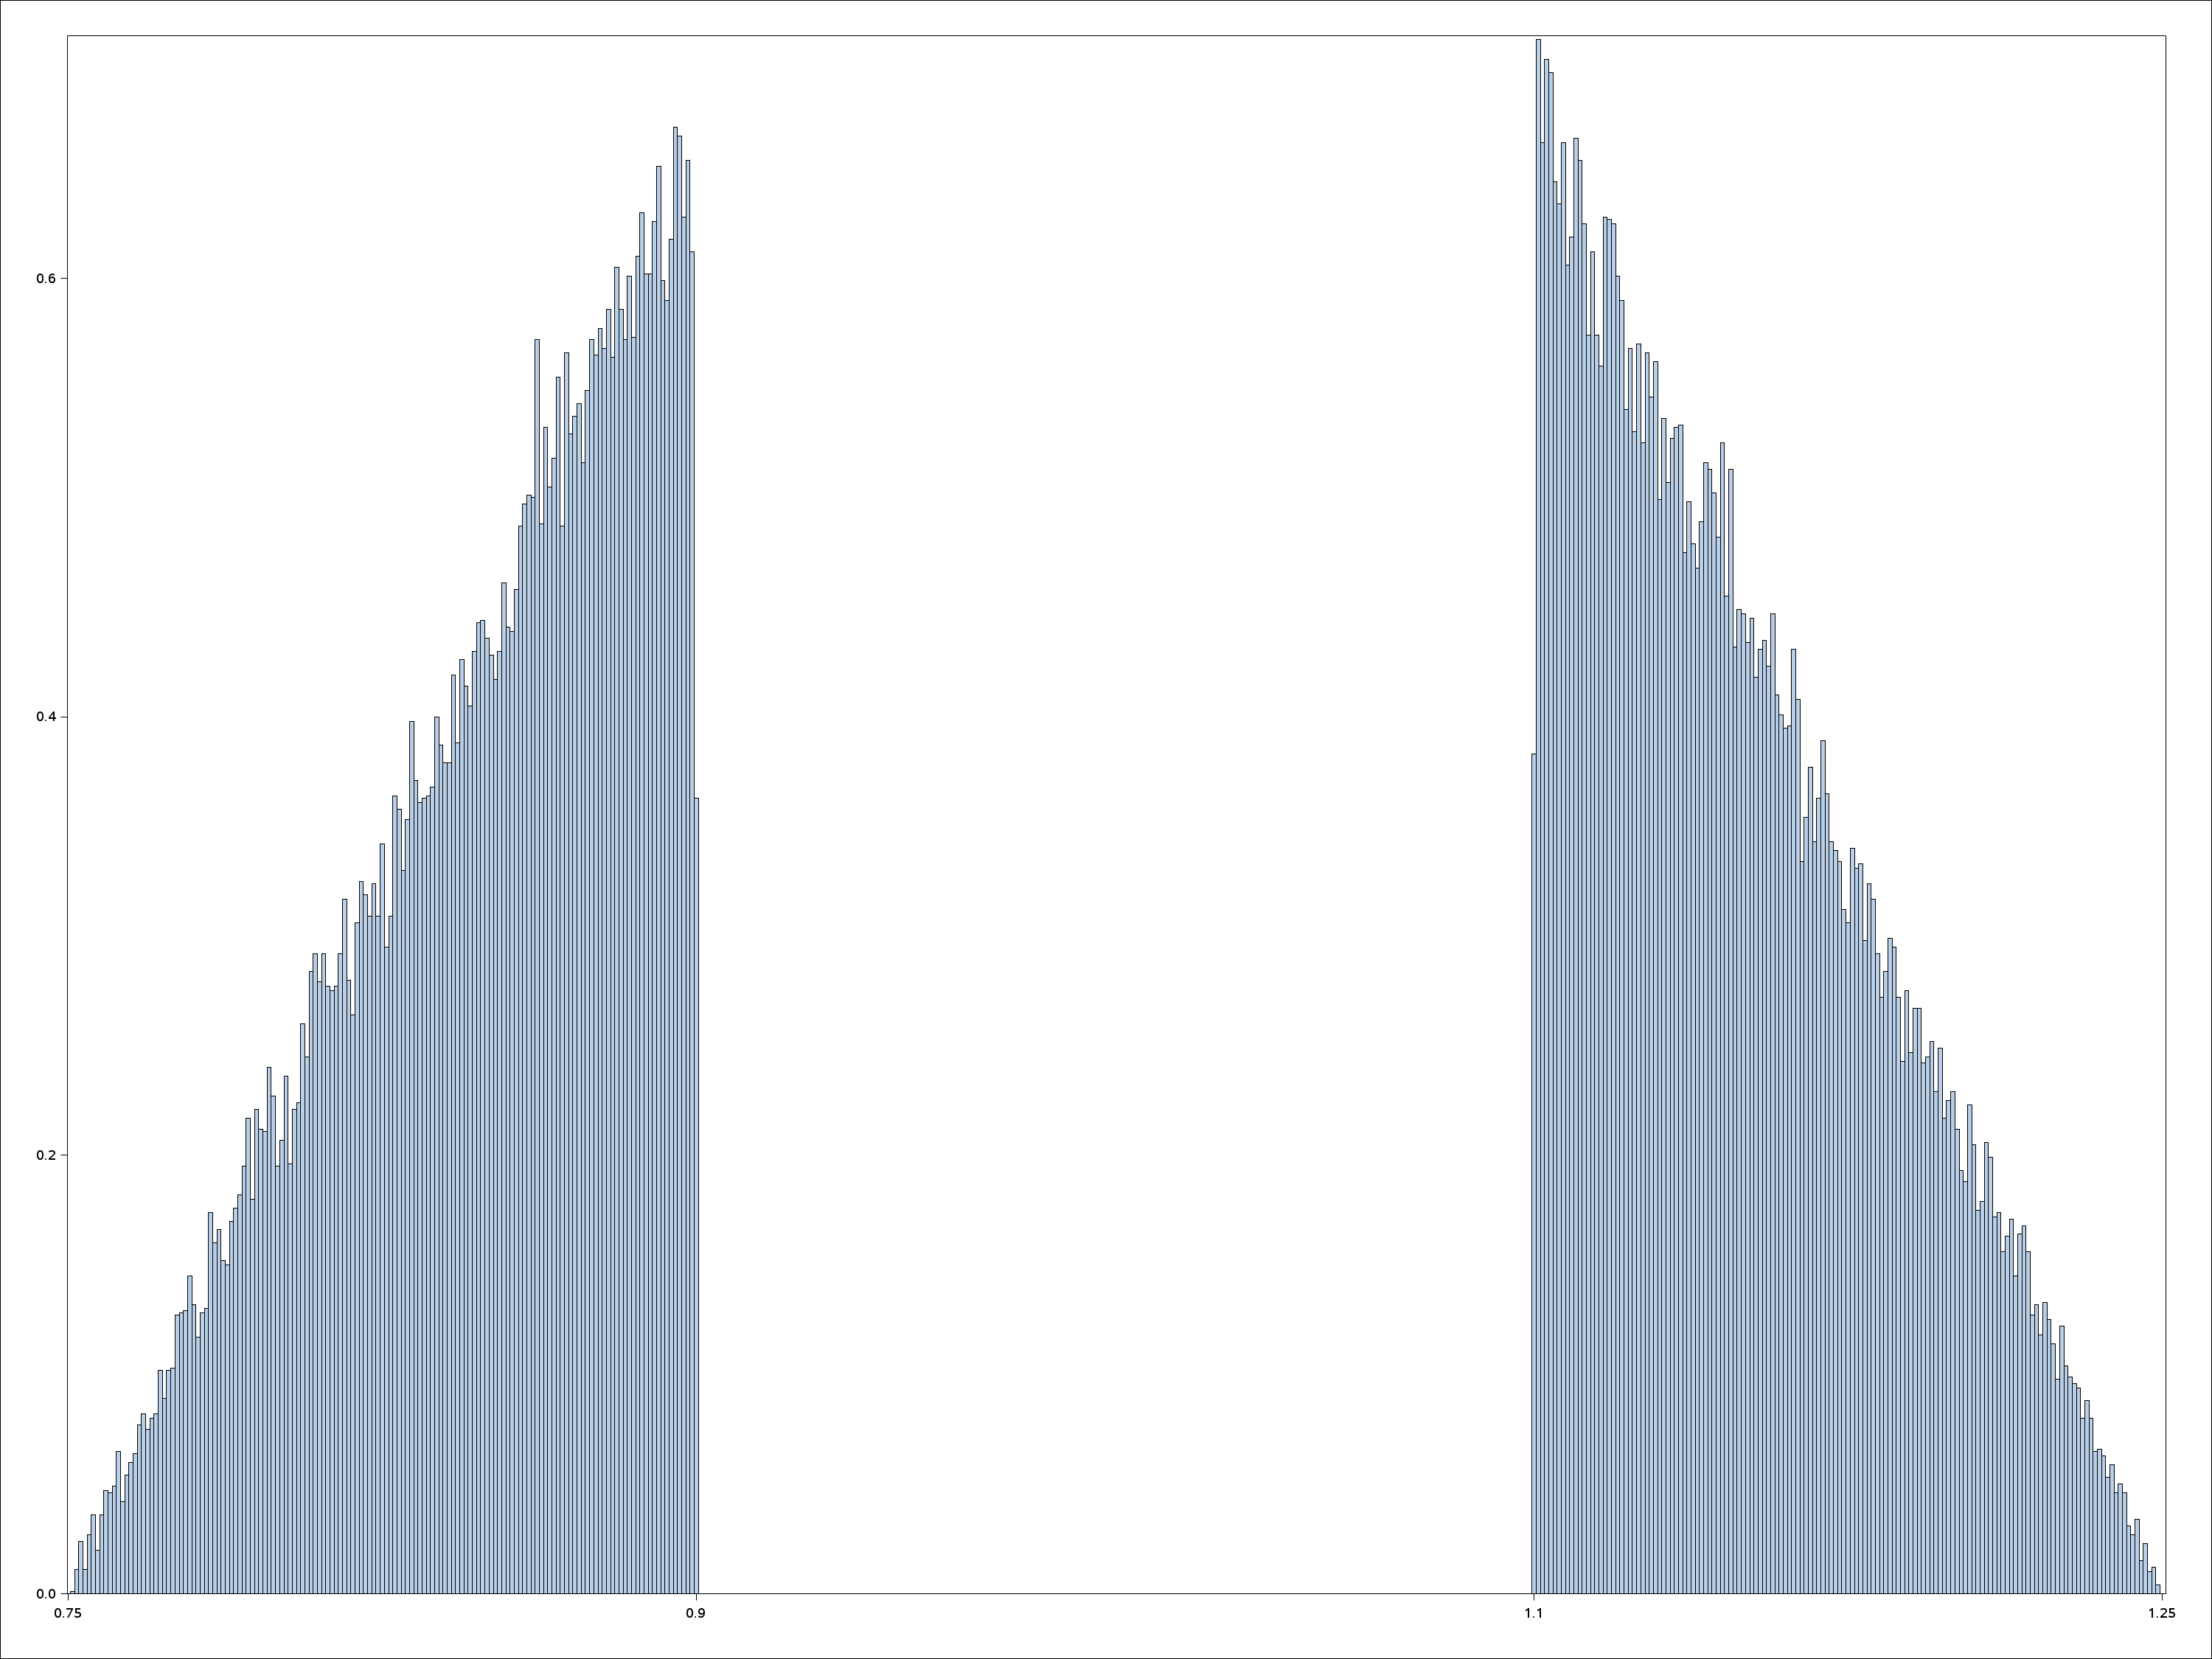
\includegraphics[width=0.5\textwidth]{SGPlot.png}
%\end{figure}



\section{Analysis}
\label{sec:analysis}
 We used \ac{SynLBD} \cite{SynLBD20}  together with confidential 
\ac{BDS} microdata (as of June 2015) for \ac{BDS} tabulations 
by establishment age and size ({\tt bds\_e\_agesz}), creating  \textbf{BDS$^{(s)}$} 
and 
\textbf{BDS$^{conf}$}, respectively. For the published data \textbf{BDS$^{(0)}$}, we used data 
from the September 2014 release. 
%\margincomment{LV}{I added this note, since it's necessary to explain the discrepancy in the estabBirths statistic - there shouldn't be any difference if really using the same input data, since there are no suppressions, but identifier corrections lead to discrepancies in that particular statistic}
We note that the \ac{BDS} microdata is thus of more recent vintage, and contains some 
improvements in the underlying data. This leads to certain discrepancies in the results, as will be 
evidenced in the tables. 
Using Algorithm~1 and combining \textbf{BDS$^{(0)}$}  and \textbf{BDS$^{(s)}$}, we created 
\textbf{BDS$^{(i)}$} and 
\textbf{BDS$^{(in)}$}. Using Algorithm~2 and combining the microdata underlying 
\textbf{BDS$^{(s)}$} 
and 
\textbf{BDS$^{conf}$}, we created \textbf{BDS$^{(ii)}$} with $n=4$, linear $w_{js}$, and $p=0$. %
%
%\footnote{$w_{j\cdot} = \left \lbrace 0, 0.2, 0.4, 0.6, 0.8 \right \rbrace$ and $\tilde{w}_{jt} = 1 - 
%w_{jt}$. }
%
Further variation of the weights $w_{js}$ and of $n$ lead to \textbf{BDS$^{(ii)}(w=0) =$  
BDS$^{(iiw)}$}%
%\footnote{$w_{j\cdot} = \left \lbrace 0, 0, 0, 0, 0 \right \rbrace$ and $\tilde{w}_{jt} = 1 - w_{jt}$. }  
 and 
\textbf{BDS$^{(ii)}(n=0) =$ BDS$^{(iin)}$}, %
%\footnote{$w_{j\cdot} = \left \lbrace 0, 1, 1, 1, 1 \right \rbrace$ and $\tilde{w}_{jt} = 1 - w_{jt}$. }  
respectively. We create \textbf{BDS$^{(n)}$} with $c=10$ and $d=25$ percent the brackets of the noise distribution.


The analysis is restricted to 1977-1999 because \ac{SynLBD} version 2.0 is only available through 
2001, and we chose to avoid any issues at the boundaries of the data. %\margincomment{Lars}{Why did I choose 1999 and not 2001?}
%
As noted in Table~\ref{tab:bds_e}, about 26\% of all cells in publicly available 
\textbf{BDS$^{(0)}$} 
have some 
suppression. For this version of the paper, we analyzed two variables, ``Job Creation by 
establishment births'' ({\tt job\_creation\_births}) and ``Job Creation by 
continuing establishments'' ({\tt job\_creation\_continuers}). Other variables, such as the 
number of establishments ({\tt estabs}) and ``Employment'' ({\tt emp}), which are never 
suppressed, 
serve as a benchmark.

\subsection{Extent of protection}
\label{sec:protection}
\input{protection}
Protection of the table relies in large part on the fact that the data replacing the suppressions is 
itself synthetic, and released (in the case of the examples in this paper) or (potentially) 
releasable (for tabulations with geography) to a broad audience \cite{AbowdVilhuber2010}. No 
establishment's observed data is released in the SynLBD, and only the industry distribution of 
establishments is preserved exactly.%
%
\footnote{To be precise, the number of establishments that ever exist within each 3-digit 
\ac{SIC} throughout the timeframe of the synthesis is preserved exactly. At any given point of 
time, though, that number will diverge from the confidential number. }
%
 A detailed analysis, based in part on a comparison of the 
confidential and synthetic microdata is 
provided elsewhere \cite{KinneyEtAl2011}. Very few synthetic values are close to the 
corresponding confidential values, and \cite{KinneyEtAl2011} conclude that the synthetic 
microdata is not disclosive of the confidential microdata. It follows that tabulations of 
non-disclosive microdata are themselves not disclosive.

We do, however, note that one particular attribute present on the confidential microdata - 
geography - was not included on the released synthetic microdata. Several of the tabulations 
listed in Table~\ref{tab:bds_e} and~\ref{tab:bds_f} are cross-tabulated by geography. Two 
options thus arise: (i) to release a version of the SynLBD with protected geography (see 
ongoing work \cite{KinneyEtAl2013}), and then use that version for tabulations; (ii) to 
create a non-released version of the SynLBD that may not satisfy the criteria for release at the microdata level, but does allow for the computation of releasable tabulations. Neither of these options are explored in the present article.

\subsection{Aggregate differences}

The present version of the \ac{SynLBD}, created in 2011, has some small aggregate differences with the released 
\ac{BDS} tables. Our analysis will not take any particular measures to alleviate the bias. 
Figure~\ref{fig:level_denom} shows  aggregated \texttt{denom} (average employment), job 
creation, and job creation by establishment births and continuing establishments, and 
Figure~\ref{fig:pct_denom} presents the percentage difference between the released data and 
the synthetic data at the most aggregated level, for the same variables. We note that 
whereas total employment is only marginally lower in the synthetic data at any point in time, synthetic job creation is significantly higher. The 
synthetic data underestimates job creation by establishment births, and overestimates job 
creation by continuing establishments. These points were originally highlighted elsewhere 
\cite{KinneyEtAl2011}, and are being addressed in the next iteration of the \ac{SynLBD}.
%\margincomment{LV}{This could still use a comparison of the Algorithm 2 final output datasets}


%\begin{figure}
%	\centering
%	\caption{Levels of released and synthetic data\label{fig:level_denom}}
%	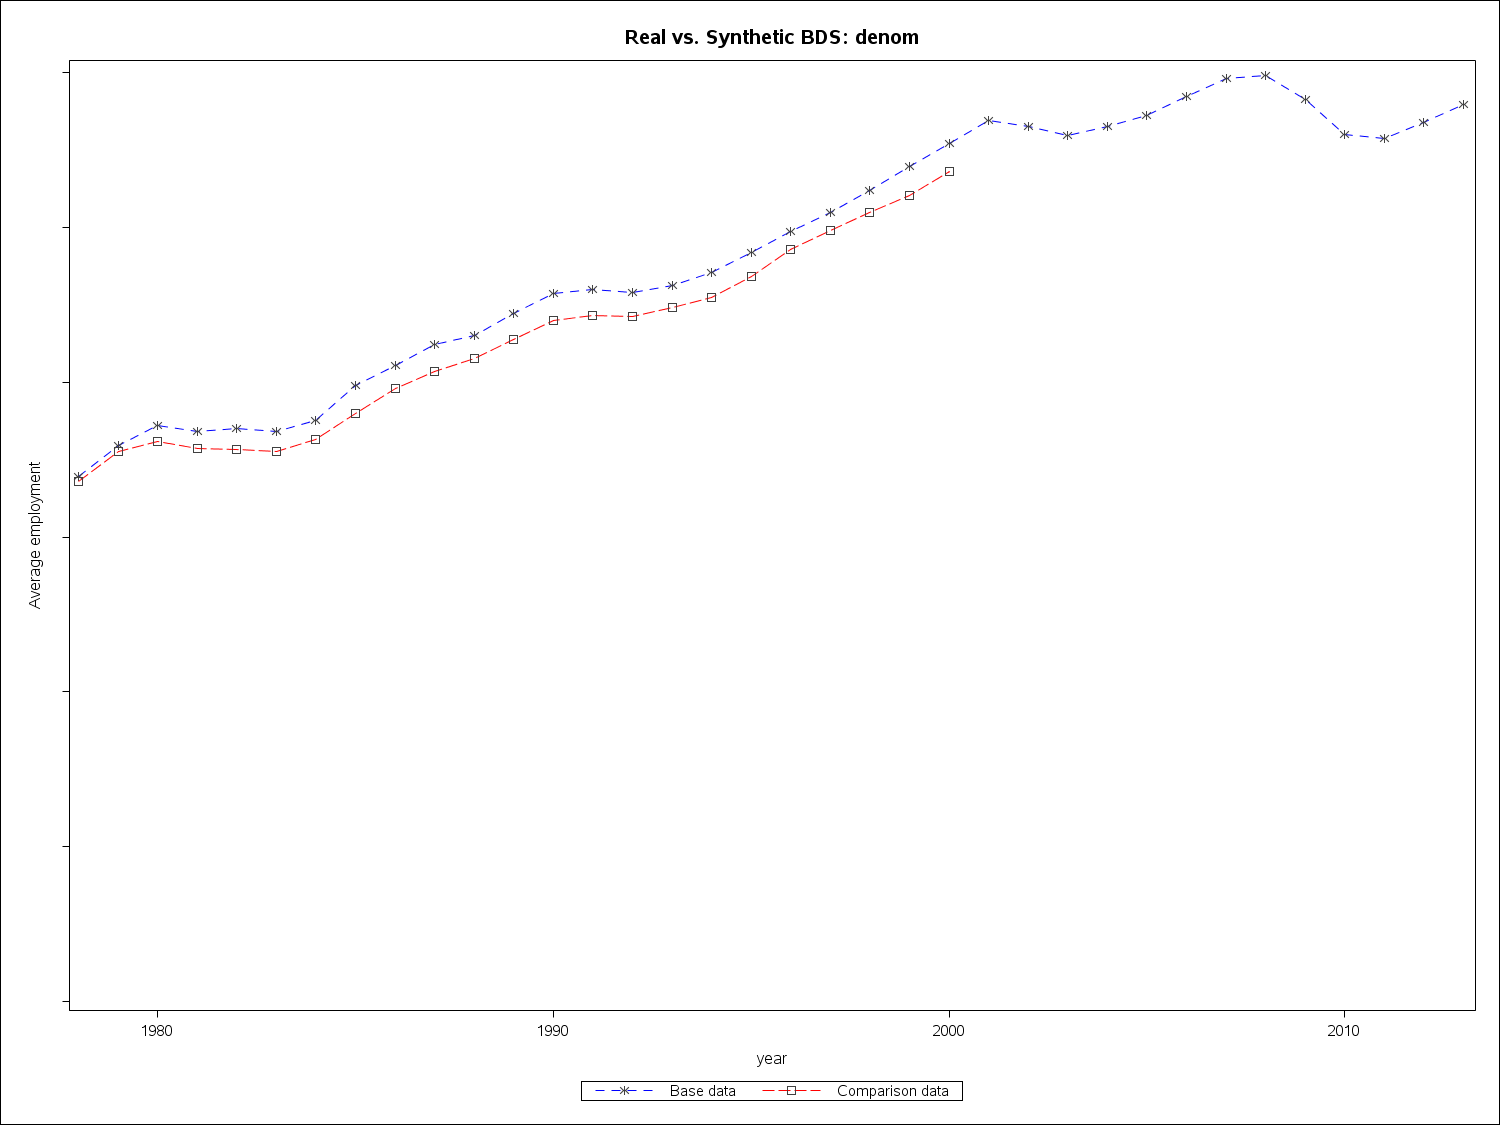
\includegraphics[width=0.45\textwidth]{results/graph_bds_real_vs_syn_denom}
%	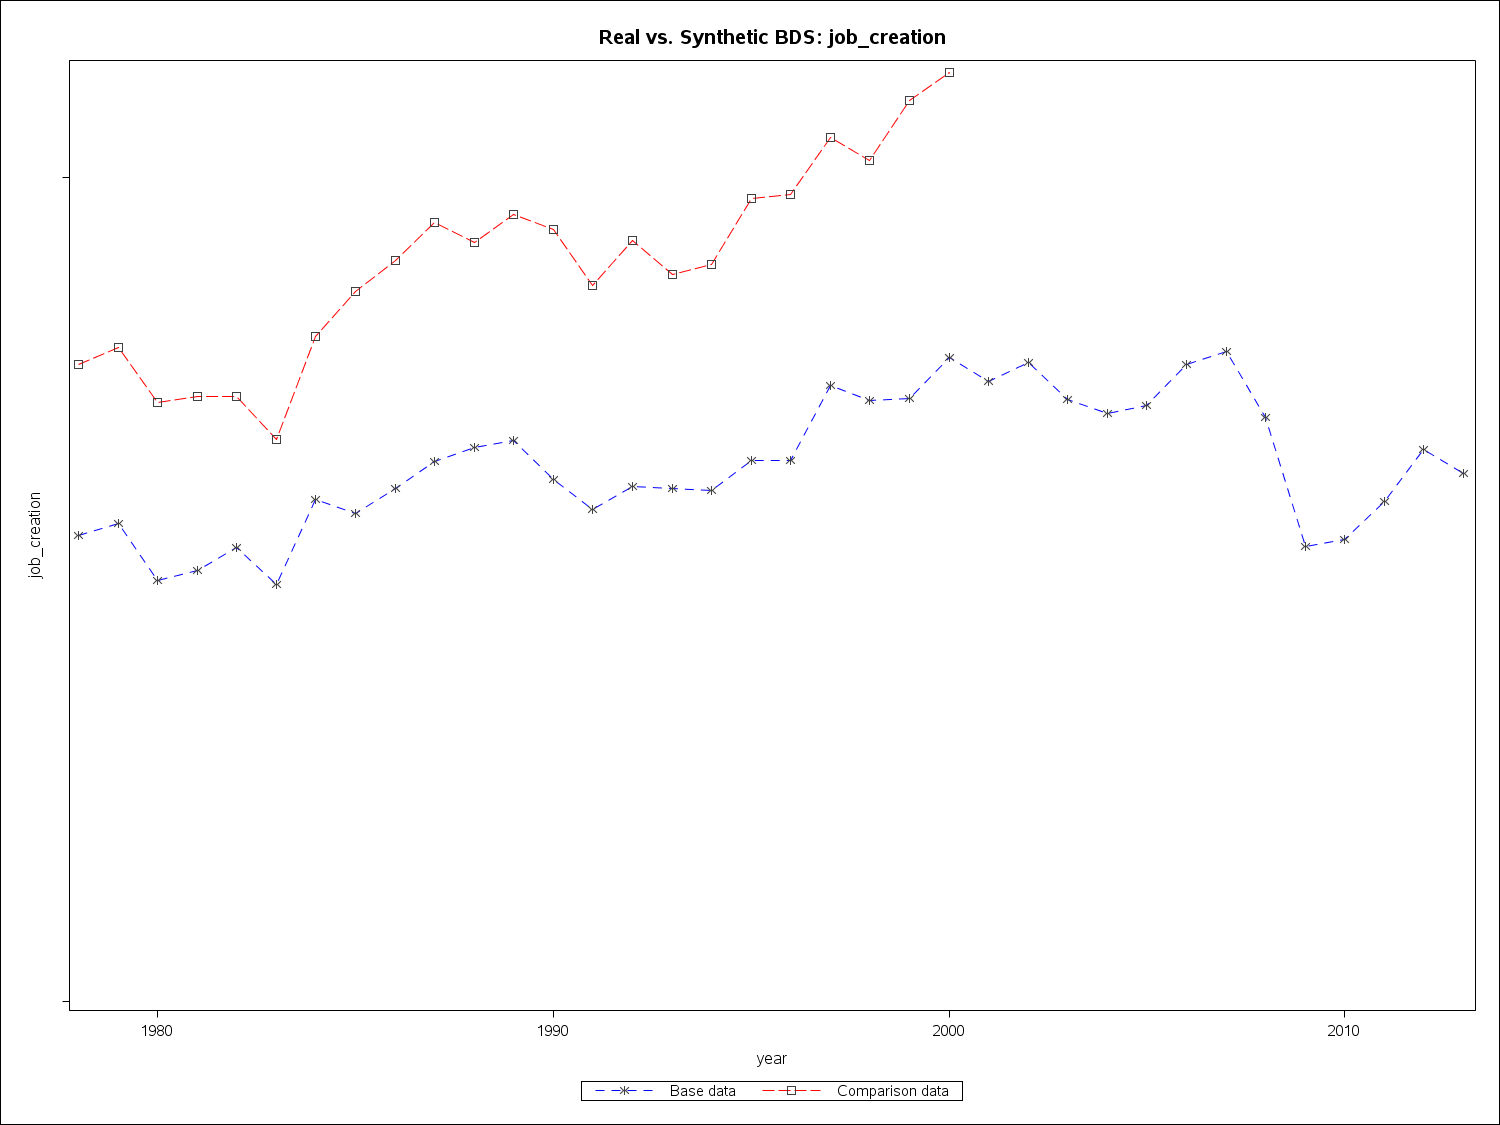
\includegraphics[width=0.45\textwidth]{results/graph_bds_real_vs_syn_job_creation}
%	
%	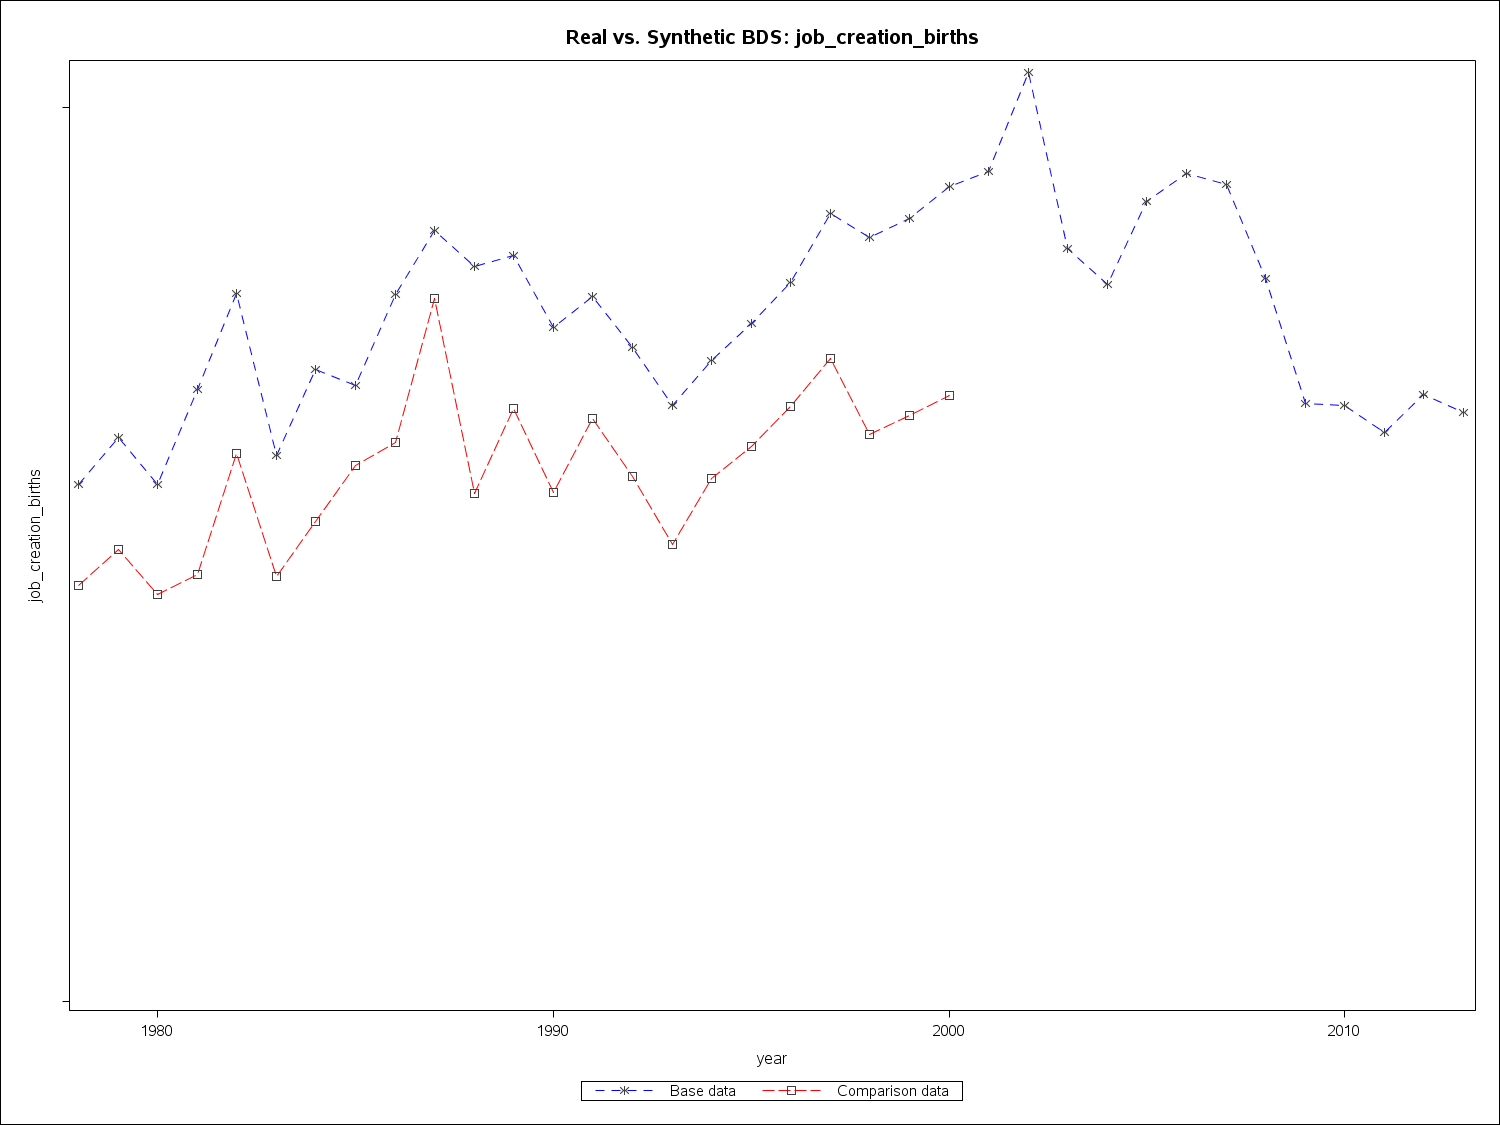
\includegraphics[width=0.45\textwidth]{results/graph_bds_real_vs_syn_job_creation_births}
%	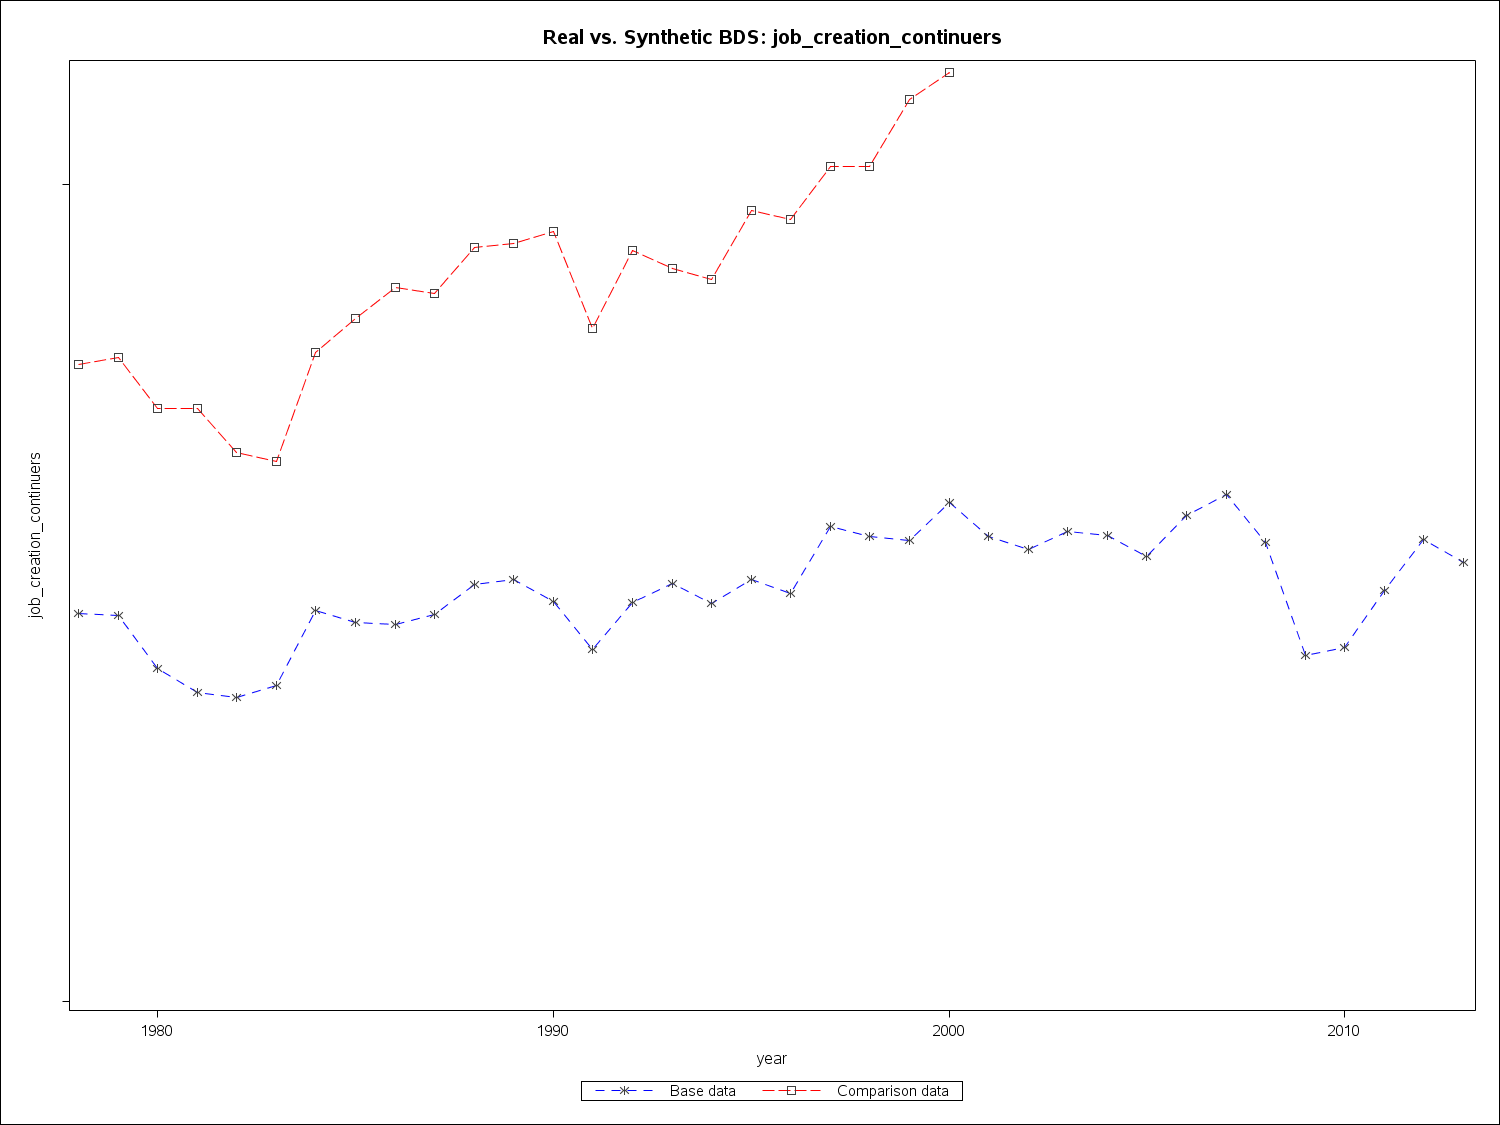
\includegraphics[width=0.45\textwidth]{results/graph_bds_real_vs_syn_job_creation_continuers}
%\end{figure}
%
%
%\begin{figure}
%\centering
%\caption{Differences between released and synthetic data\label{fig:pct_denom}\label{fig:pct_jc}}
%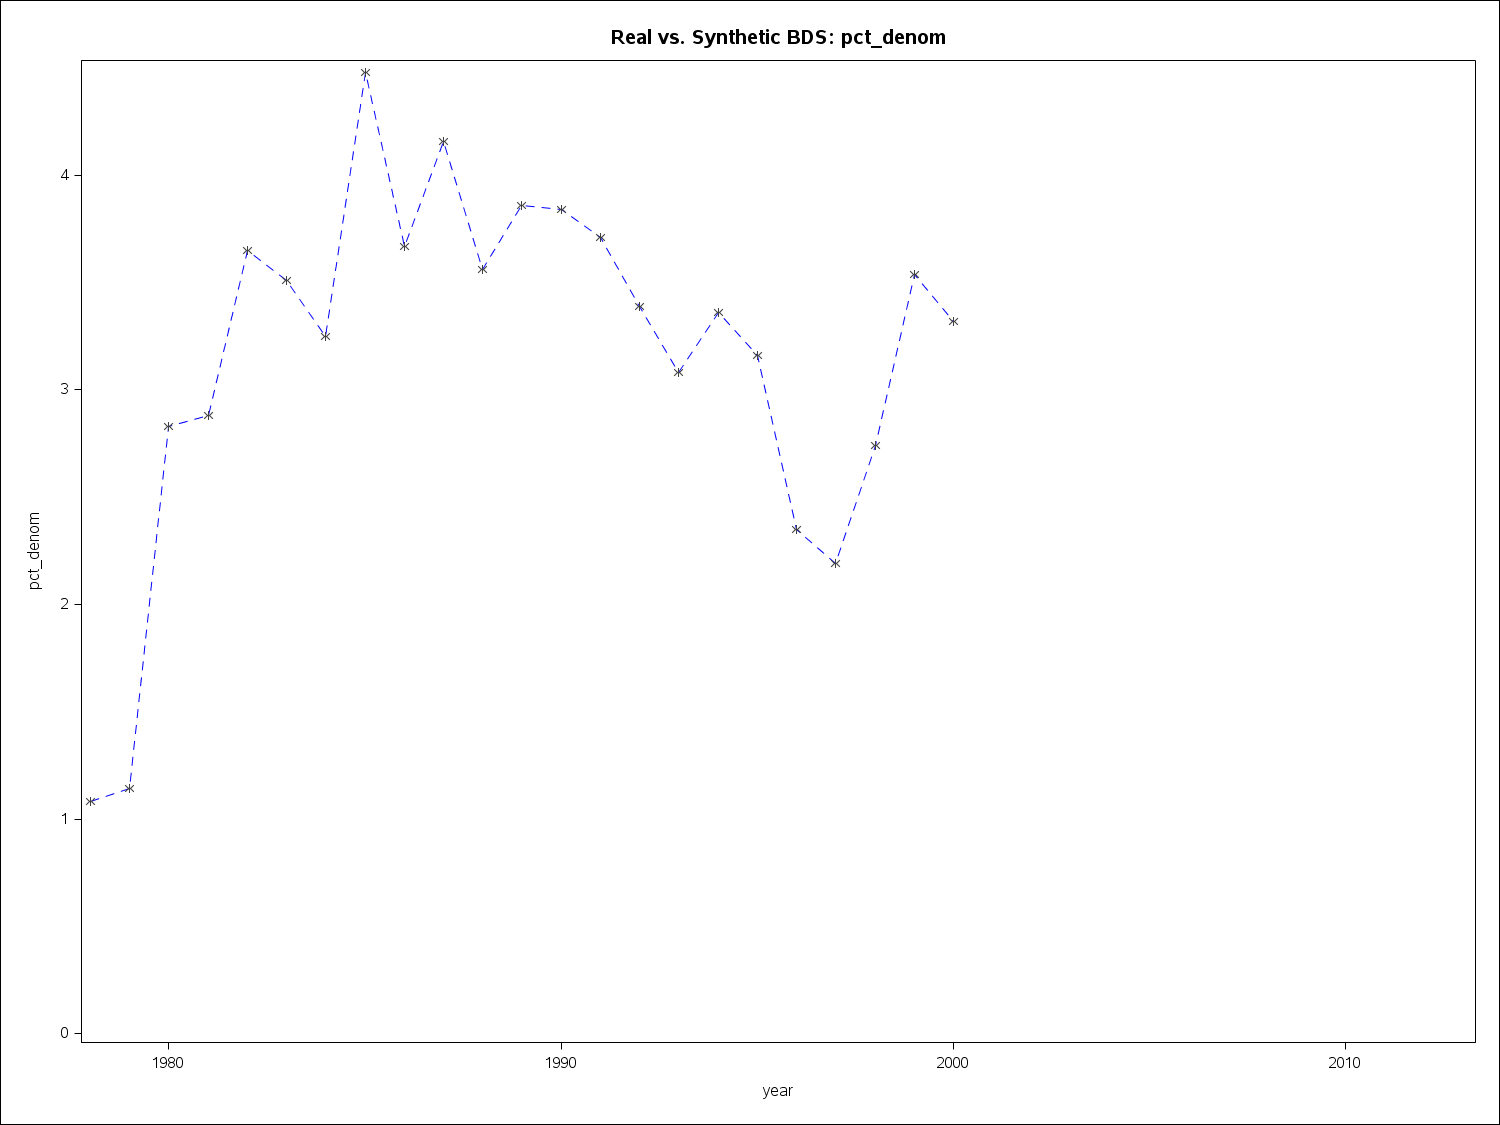
\includegraphics[width=0.45\textwidth]{results/graph_bds_real_vs_syn_pct_denom}
%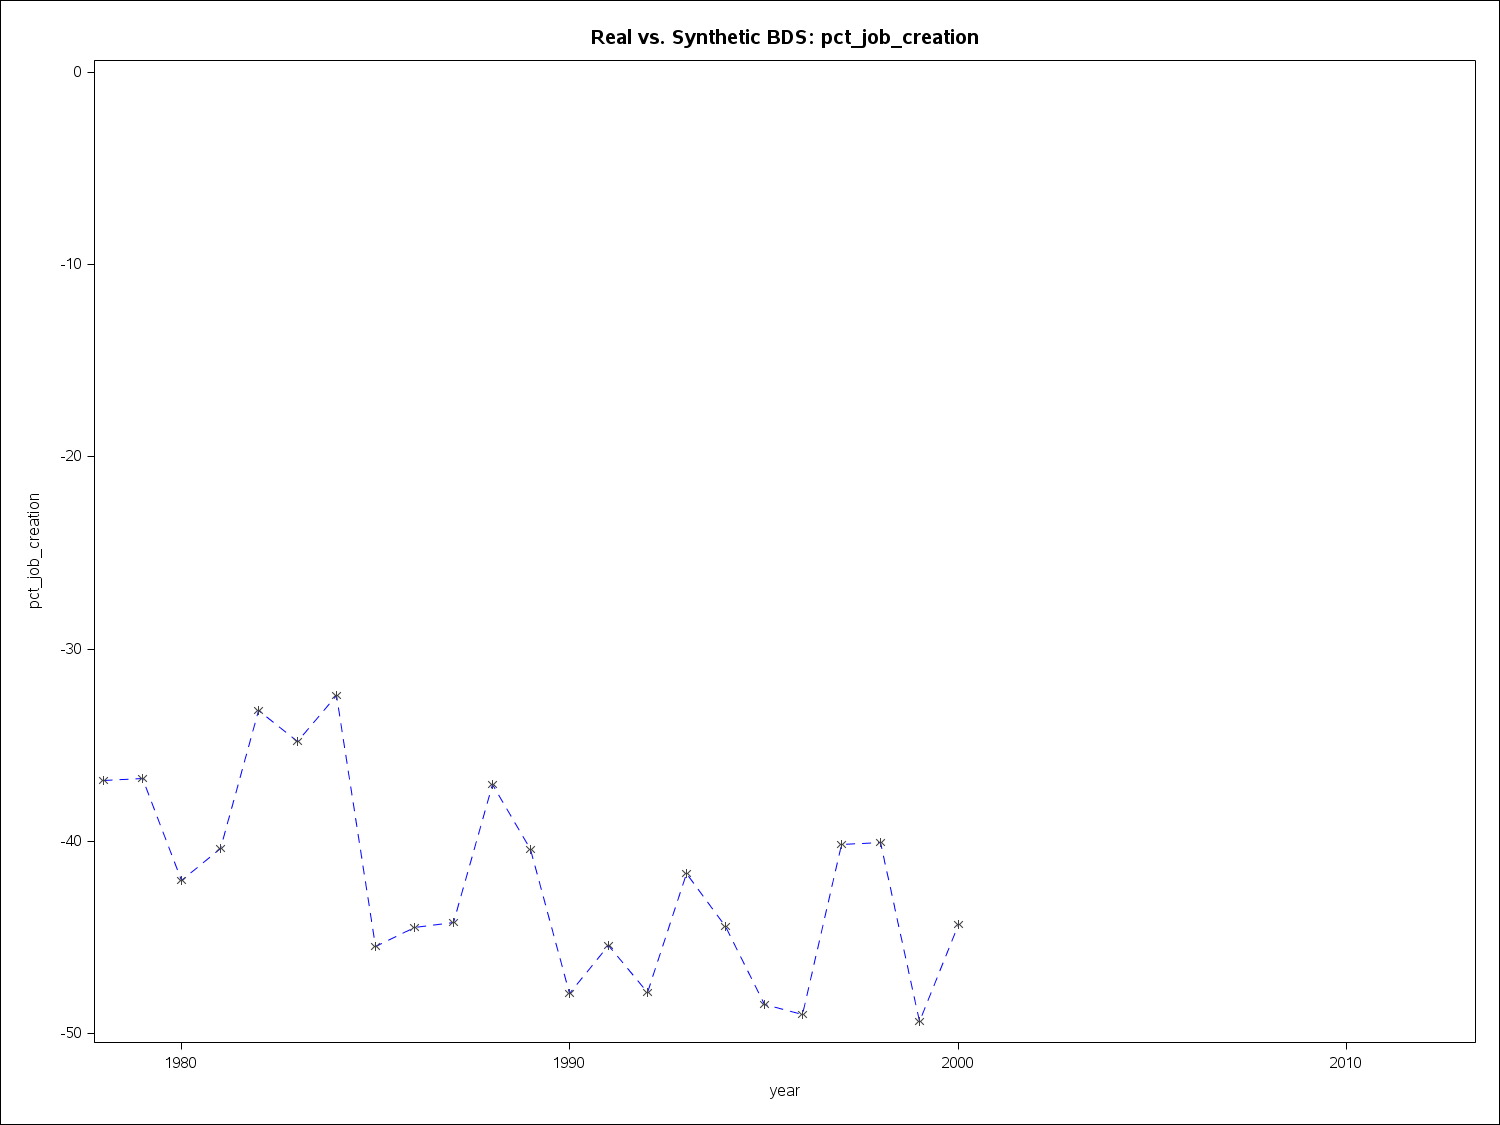
\includegraphics[width=0.45\textwidth]{results/graph_bds_real_vs_syn_pct_job_creation}
%
%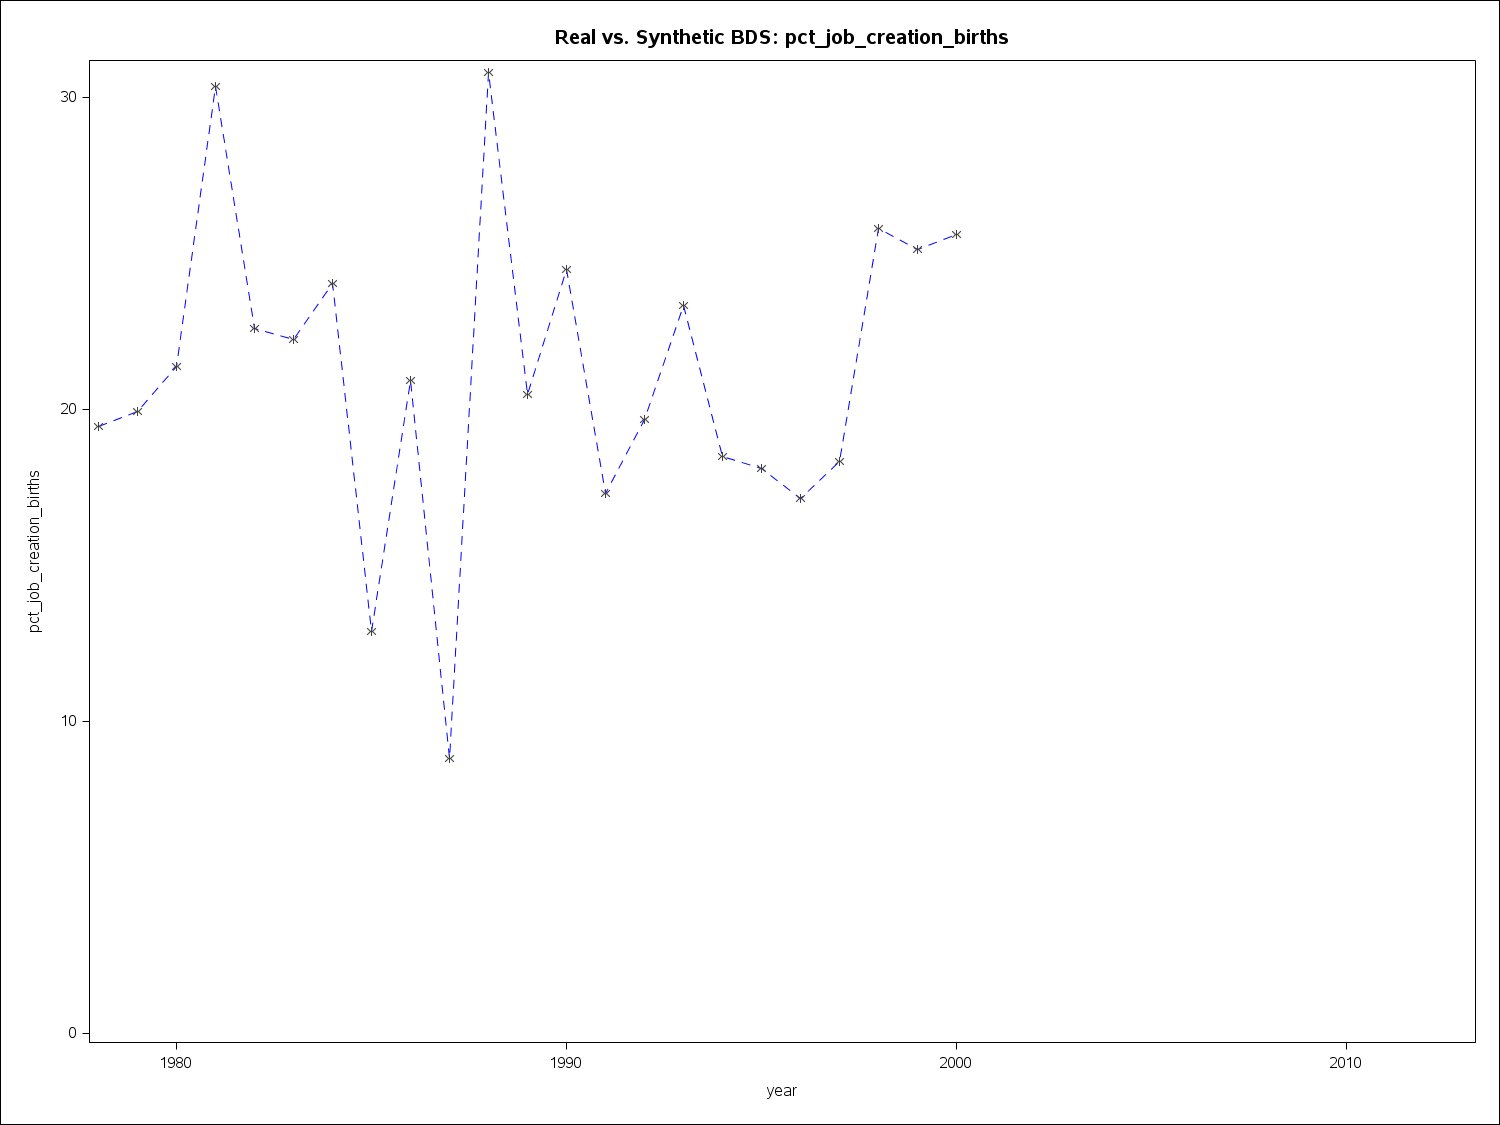
\includegraphics[width=0.45\textwidth]{results/graph_bds_real_vs_syn_pct_job_creation_births}
%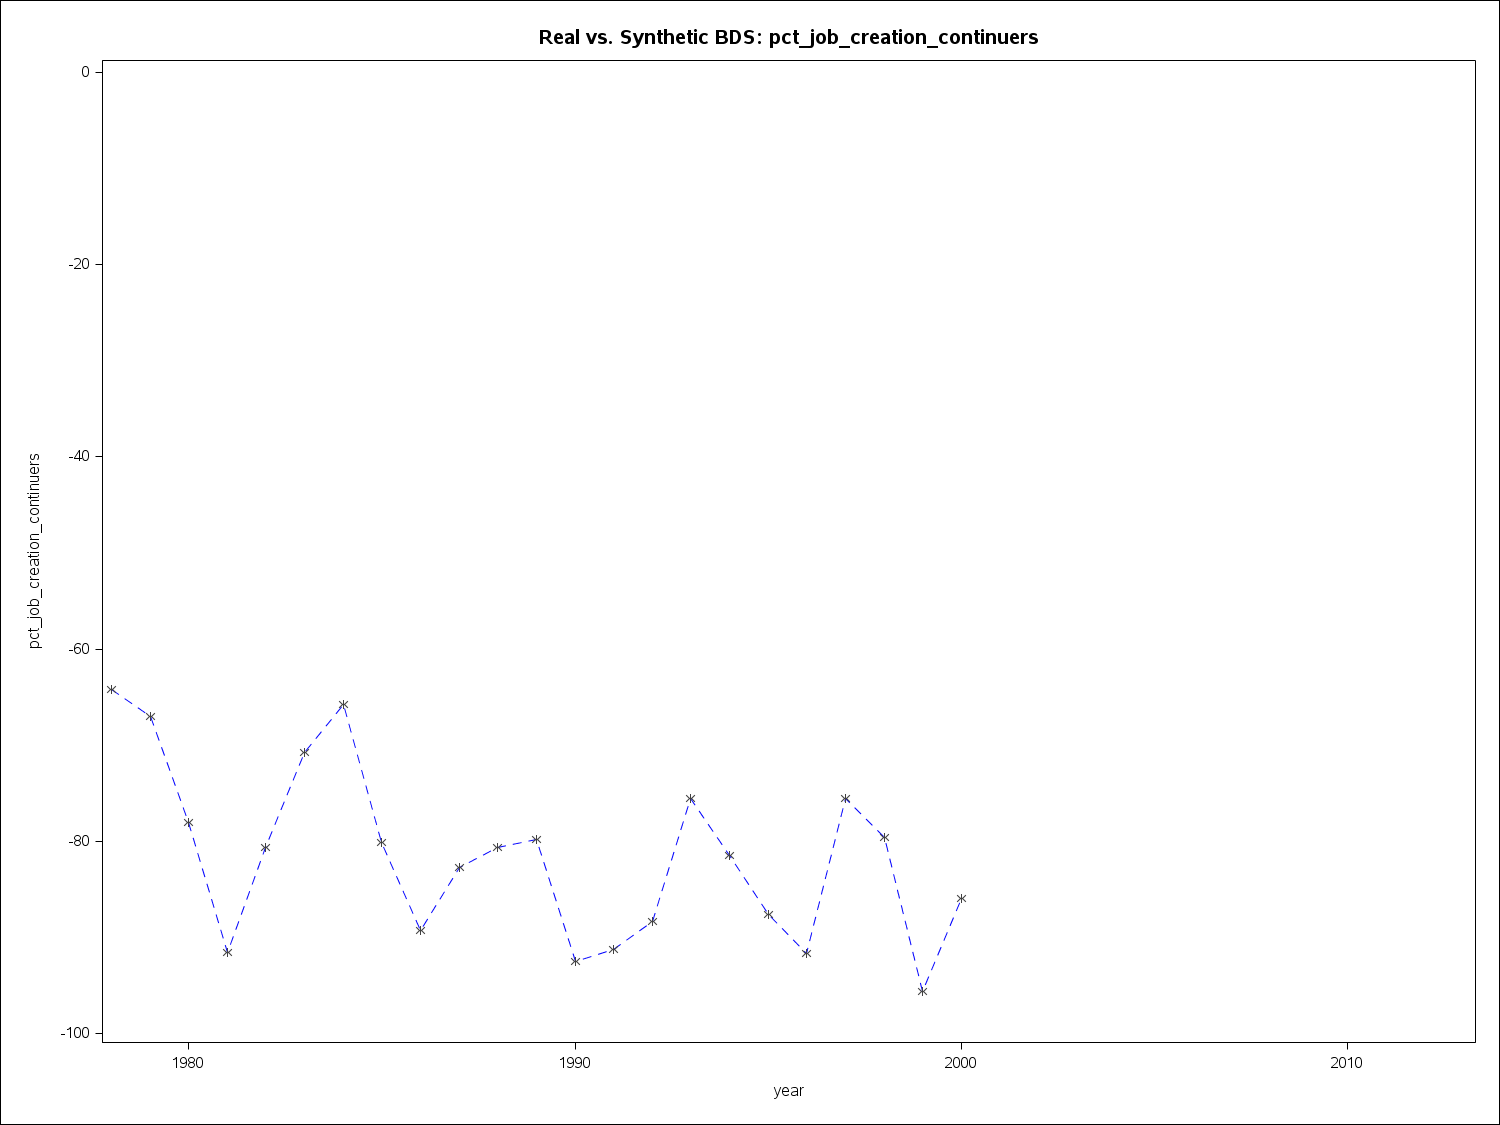
\includegraphics[width=0.45\textwidth]{results/graph_bds_real_vs_syn_pct_job_creation_continuers}
%\end{figure}


For comparison, there are no such differences at the most aggregated level between releasable and noise-infused tabulations (not shown). Percentage differences are less than two-tenths of a percent in all cases, as expected. 

%Section~\ref{sec:synthetic_method}, Table~TBD provides a 
%transition matrix for small values of the (confidential) $X_{k^\prime t}$ against $X_{k^\prime 
%t}^{s}$, $X_{k^\prime t}^{(i)}$, and 
%$X_{k^\prime t}^{(ii)}$, for several variables of interest (establishment births and deaths, job 
%creation and destruction, employment levels). (Table~TBD is being computed and/or pending 
%release at the time of submission of this document).

\subsection{Analytical validity}
%\margincomment{LARS}{We need to redo the histogram from Kinney et al (differences at the estab level) - can we (merge by LBDID)? Then need to do the same analysis, but at the cell level - histogram of differences in affected cells - those with suppressions/filled in, and the ancillary cells (t+1 through t+p) that are affected by the smoothing}
\label{sec:validity}
We turn to an assessment of analytical validity. In order to assess the analytical validity of each of 
the methods, we focus on simple 
%\margincomment{Lars}{cross-sectional distributional properties as well as }
time-series 
properties of  the $X_{k^\prime t}$. 
%\margincomment{Lars}{::For the cross-section, we compute for each year the Jenson-Shannon Divergence (JSD) metric for the entire table, and for those cells that ...:: HOW TO COMPUTE JSD when cells are missing?}
In particular, we 
estimate a AR(2) process for each of time-series generated by 
$X_{k^\prime t}$, $X_{k^\prime t}^{(0)}$, $X_{k^\prime t}^{(s)}$,  $X_{k^\prime t}^{(i)}$, $X_{k^\prime t}^{(ii)}$,   
$X_{k^\prime t}^{(iiw)}$, and $X_{k^\prime t}^{(iin)}$. 
We then assess, for each statistic $X$ under each of the regimes, the number of feasible regressions for $X_{k^\prime t}$ (for some values of $k$, data points may be missing because out-of-scope in certain time periods), and what fraction of the feasible regressions can be replicated under the alternate regimes. Table~\ref{tab:bds_e_pctmiss} presents these results for a number of variables.
%\margincomment{LV}{Table 3 would probably be better as a graph}
Conditional on a feasible estimation, we tabulate the fraction of $\rho_1$ estimates that are 
statistically significant at conventional levels (Table~\ref{tab:bds_e_pctmiss}).


%\begin{table}[p]
		\setlength{\tabcolsep}{6pt}
\caption{Analytic validity: Feasibility of AR(2) regressions \label{tab:bds_e_pctmiss}}
\centering
%\begin{tabular}{|lc|r|rrr|}\hline%
\csvreader[tabular=|l|r|r|rrr|rrr|r|,table head=\hline 
	&Number 
	&\multicolumn{8}{c|}{Percent} 
\\
Variable 
	&feasible 
	& \multicolumn{8}{c|}{Infeasible}                
\\
    & $X_{k^\prime t}$ 
    & $X_{k^\prime t}^{(s)}$ 
    & $X_{k^\prime t}^{(0)}$ 
    & $X_{k^\prime t}^{(i)}$
    & $X_{k^\prime t}^{(in)}$
    & $X_{k^\prime t}^{(ii)}$
    & $X_{k^\prime t}^{(iiw)}$
    & $X_{k^\prime t}^{(iin)}$
    & $X_{k^\prime t}^{(n)}$
    \\\hline,
	late after line=\\,late after last line=\\\hline]%
{results/r_e_agesz_all_missing.csv}{Variable=\V,number=\colz,missing1=\cola,missing2=\colb,missing3=\colc,missing4=\cold,missing5=\cole,missing6=\colf,missing7=\colg,missing8=\colh}%
{\V &  \colz & \cola & \colb & \colc & \cold & \cole & \colf & \colg &\colh}%
\end{table}

%\begin{table}[p]
	\setlength{\tabcolsep}{6pt}
\caption{Analytic validity: AR(2) regressions with significant parameters\label{tab:bds_e_pctsign}}
\centering
%\begin{tabular}{|lc|r|rrr|}\hline%
\csvreader[tabular=|l|rr|rrr|rrr|r|,table head=\hline 
	& \multicolumn{9}{c|}{Percent} 
\\
Variable 
	& \multicolumn{9}{c|}{significant}
\\
    & $\rho_{1}$ 
    & $\rho_{1}^{(s)}$ 
    & $\rho_{1}^{(0)}$ 
    & $\rho_{1}^{(i)}$
    & $\rho_{1}^{(in)}$
    & $\rho_{1}^{(ii)}$
    & $\rho_{1}^{(iiw)}$
    & $\rho_{1}^{(iin)}$
    & $\rho_{1}^{(n)}$
    \\\hline,
	late after line=\\,late after last line=\\\hline]%
{results/r_e_agesz_all_significant.csv}{Variable=\V,significantconf2=\colz,significant1=\cola,significant2=\colb,significant3=\colc,significant4=\cold,significant5=\cole,significant6=\colf,significant7=\colg,significant8=\colh}%
{\V &  \colz & \cola & \colb & \colc & \cold & \cole & \colf & \colg &\colh }%
\end{table}


Two measures of utility are also computed.
We compute \emph{coverage} as the 
percentage of regressions where the true $\rho_1$ lies within the confidence band around the 
coefficient estimated from the comparison $\rho_1^{*}$ for each of the tables generated by the 
different algorithms. Let $(L^{*},U^{*})$ be the 95\% confidence interval for $\rho_1^{*}$. 
\emph{Coverage} is the percentage of AR(2) estimates for which the ``true'' $\rho_1 \in  
(L^{*},U^{*})$. We 
generalize this measure  as suggested by \cite{tas2006}, and compute  the \emph{interval 
overlap measure} $J_k$. Consider the overlap of confidence intervals $(L,U)$ for $\rho_1$ (estimated from the confidential data) and $(L^{*},U^{*})$ for $\rho_1^*$. Let $L^{over} = \max (L,L^{*} )$ and $U^{over} = \min (U,U^{*})$. Then the average overlap in confidence intervals is

$$
J_k^{*} = \frac{1}{2} \left [ \frac{U^{over} - L^{over}}{U-L} + \frac{U^{over} - L^{over}}{U^*-L ^*}        \right ]
$$
We then average $J_k^{*}$ over all estimated AR(2) regressions.
Results are summarized in Tables~\ref{tab:bds_e_coverage} and \ref{tab:bds_e_jk}.

%\begin{table}[p]
		\setlength{\tabcolsep}{6pt}
\caption{Analytic validity: AR(2) regressions: 
Coverage\label{tab:bds_e_coverage}}
\centering
%\begin{tabular}{|lc|r|rrr|}\hline%
\csvreader[tabular=|l|r|rrr|rrr|r|,table head=\hline 
	& \multicolumn{8}{c|}{} 
\\
Variable 
	& \multicolumn{8}{c|}{Coverage}
\\
    & $\rho_{1}^{(s)}$ 
    & $\rho_{1}^{(0)}$ 
    & $\rho_{1}^{(i)}$
    & $\rho_{1}^{(in)}$
    & $\rho_{1}^{(ii)}$
    & $\rho_{1}^{(iiw)}$
    & $\rho_{1}^{(iin)}$
    & $\rho_{1}^{(n)}$
    \\\hline,
	late after line=\\,late after last line=\\\hline]%
{results/r_e_agesz_all_coverage.csv}{Variable=\V,coverage1=\cola,coverage2=\colb,coverage3=\colc,coverage4=\cold,coverage5=\cole,coverage6=\colf,coverage7=\colg,coverage8=\colh}%
{\V &  \cola & \colb & \colc & \cold & \cole  & \colf & \colg &\colh}%
\end{table}

%\begin{table}[p]
			\setlength{\tabcolsep}{6pt}
\caption{Analytic validity: AR(2) regressions: Interval 
overlap\label{tab:bds_e_jk}}
\centering
%\begin{tabular}{|lc|r|rrr|}\hline%
\csvreader[tabular=|l|r|rrr|rrr|r|,table head=\hline 
	& \multicolumn{8}{c|}{Interval} 
\\
Variable 
	& \multicolumn{8}{c|}{overlap}
\\
    & $J_k^{(s)}$ 
    & $J_k^{(0)}$ 
    & $J_k^{(i)}$
    & $J_k^{(in)}$
    & $J_k^{(ii)}$
    & $J_k^{(iiw)}$
    & $J_k^{(iin)}$
    & $J_k^{(n)}$
    \\\hline,
	late after line=\\,late after last line=\\\hline]%
{../results/r_e_agesz_all_Jk.csv}{Variable=\V,Jk1=\cola,Jk2=\colb,Jk3=\colc,Jk4=\cold,Jk5=\cole,Jk6=\colf,Jk7=\colg,Jk8=\colh}%
{\V &  \cola & \colb & \colc & \cold & \cole & \colf & \colg &\colh}%
\end{table}


%\margincomment{LV}{This whole section is new.}
We start by noting issues surrounding establishment births in both the synthetic and different 
releases of the observed data. Establishment births are particularly sensitive to identifier 
linkages, and regular improvements to the BDS microdata occur. On the other hand, it is one of 
the more difficult events to synthesize. This leads to discrepancies both between the synthetic 
and the confidential data, and between the public-use data released in September 2014 and the 
(preliminary) confidential tabulations from the June 2015 BDS microdata. 

We further note that the first two rows of each table serve as a control, reporting results for 
\textbf{emp} and 
\textbf{estabs}, never show any differences, since there are no observed suppressions. Job 
creation, which also is never suppressed, does show some differences in 
Table~\ref{tab:bds_e_jk} between \textbf{BDS$^{(0)}$} and \textbf{BDS$^{conf}$}, presumably 
due to data revisions.

Tables~\ref{tab:bds_e_coverage} and~\ref{tab:bds_e_jk} paint approximately the same picture. 
The synthetic data is sufficiently different to distort inferences in our application further away 
from the results obtained from the confidential data. While the published data, despite having 
suppressed cells, has an average $J_k$ of 92.6\%, filling in suppressions together with smoothing 
($n=4$) yields an average $J_k$ of 77.5\%. Clearly this is being driven by the increased use of 
statistically different synthetic data, since setting $n=0$ (and thus using less synthetic data in the 
tabulations) yields a higher average $J_k$. The results obtained through Algorithm~2 are 
qualitatively better, with very little variation across the parameter variations. Given the data 
vintage differences noted above, it is not reasonable to compare $J_k^{(0)}$ and $J_k^{(ii)}$ 
directly until consistent input data can be used.





\section{Concluding remarks}
\label{sec:conclusion}
In this paper, we have described several alternate mechanisms to substitute for suppressions in  small-cell tabulations of business 
microdata, with the goal of improving analytic validity while maintaining a sufficiently high 
standard of disclosure limitation. Neither mechanism fundamentally changes the existing 
suppression methodology, rather, the mechanisms work to fill in the holes created by the 
suppression methodology. In particular, the first methodology (Algorithm 1) can be used 
ex-post, after initial publication of tabulations with cell suppressions. 

Leveraging the availability of a high-quality synthetic dataset
(the Synthetic LBD) with proven disclosure limitation efficiency and analytic validity \cite{KinneyEtAl2011}, the first 
method is very simple, but may suffer from seam biases and time-inconsistency. The second 
method aims to improve on that by ``blending in'' real establishments after the need for suppressions has disappeared, which may slightly 
reduce analytic validity in time periods where the strict application of the suppression 
algorithms would no longer impose any constraints, but improving on the time-series properties 
of the released data. 

%\margincomment{LV}{This section added.}
For reference, we have also used a noise-infused version of the BDS, and performs similarly if not better. 

The (preliminary) results do not bear out our hypothesis that the use of microdata for 
prolonged periods of time improves the analytic validity of the data. However, we refrain from 
definitive conclusions at this time, due to differences in the underlying microdata that 
contaminate the current results. Current improvements in the upcoming next release of both 
the existing BDS (expected in late 2015) and a new release of the Synthetic LBD will need to be 
incorporated for a more consistent analysis. Clearly, the success of our proposed methods 
depends heavily on the analytic validity of the underlying synthetic data being used.

Recent developments to improve the micro-level analytic validity of the 
\ac{SynLBD} \cite{CES-WP-2014-12} should improve the analytic validity of the mechanisms 
proposed here as well.  We also compare our proposed mechanisms to the actual published, but otherwise unmodified \ac{BDS}. Comparing  post-publication improvements to a table with suppressions \cite{HolanEtAl2010} will inevitably lead to an apparent reduction in the utility of this particular approach. Finally, the approach relies on continuous availability of synthetic microdata with analytical validity. Other approaches rely on fewer data points, and thus may be favored due to lower implementation costs.





%\newpage
\subsubsection*{Acknowledgments.} 
\label{sec:ack}
% $Id: acknowledgements.tex 1695 2015-07-23 02:10:46Z lv39 $
% $URL: https://forge.cornell.edu/svn/repos/lv39_papers/SynLBD/text/JSM2015/acknowledgements.tex $

Vilhuber acknowledges support through NSF Grants SES-1042181 and BCS-0941226. We thank 
Jorgen Harris for 
able research assistance.
This project would not have been feasible without  repeated input from Saki Kinney and Jerry 
Reiter, and their valuable work on the Synthetic LBD. 
%
\textit{Disclaimer.}
All authors were affiliated with the U.S. Census Bureau, Center for Economic Studies, when 
originally contributing to the contents of this paper. 
This document reports the results of research and analysis
undertaken by U.S. Census Bureau staff. It has undergone a Census
Bureau review more limited in scope than that given to official Census
Bureau publications. This document is released to inform interested
parties of ongoing research and to encourage discussion of work in
progress. All results have been reviewed to ensure that no confidential information is
disclosed. The views expressed herein are attributable only to the
authors and do not represent the views of the U.S. Census Bureau. 
%
\textit{Data access.}
The data used in this paper is restricted-access, and can be accessed either through the Federal 
Statistical Research Data Centers (LBD) or through the Synthetic Data Server at Cornell University 
(Synthetic LBD). Data and code used for the final version of this paper will be archived at the U.S. 
Census Bureau and made available upon request. 



\clearpage
\bibliography{abbrev,paper,theses,common-bib-ces-wp}
\bibliographystyle{vancouver}

% $Id: appendix.tex 1793 2016-01-18 18:18:16Z lv39 $
\appendix
\section*{Appendix}
%\clearpage
\section*{Ramp algorithm in SAS}
\lstinputlisting{rampdist.sas}

\clearpage
\section*{Tables}

\begin{table}
\caption{Suppressions in establishment-level BDS\label{tab:bds_e}}
\centering
\begin{tabular}{|l|r|rrr|}\hline%
               &                 \bfseries Number &\multicolumn{3}{c|}{\bfseries Suppressions (\%)}\\
\cline{3-5}
\bfseries Type  &\bfseries of     &                            & \multicolumn{2}{c|}{\bfseries Job creation}\\
\cline{4-5}
                                                          &\bfseries  cells& \bfseries Any  &\bfseries by entrants &\bfseries 
                                                          by continuers\\
\hline
\csvreader[head to column names,late after line=\\,late after last line=\\\hline]%
{programs/bds_e_suppressions_multi.csv}{}%
{\typename &  \cells & \percentsup  & \jcbirths &\jcconts}%
\multicolumn{4}{p{0.6\textwidth}}{\footnotesize Note: Cells are year $x$ categories, where the 
number of categories varies by published table.}
\end{tabular}
\end{table}

\clearpage
\begin{table}[p]
		\setlength{\tabcolsep}{6pt}
\caption{Analytic validity: Feasibility of AR(2) regressions \label{tab:bds_e_pctmiss}}
\centering
%\begin{tabular}{|lc|r|rrr|}\hline%
\csvreader[tabular=|l|r|r|rrr|rrr|r|,table head=\hline 
	&Number 
	&\multicolumn{8}{c|}{Percent} 
\\
Variable 
	&feasible 
	& \multicolumn{8}{c|}{Infeasible}                
\\
    & $X_{k^\prime t}$ 
    & $X_{k^\prime t}^{(s)}$ 
    & $X_{k^\prime t}^{(0)}$ 
    & $X_{k^\prime t}^{(i)}$
    & $X_{k^\prime t}^{(in)}$
    & $X_{k^\prime t}^{(ii)}$
    & $X_{k^\prime t}^{(iiw)}$
    & $X_{k^\prime t}^{(iin)}$
    & $X_{k^\prime t}^{(n)}$
    \\\hline,
	late after line=\\,late after last line=\\\hline]%
{results/r_e_agesz_all_missing.csv}{Variable=\V,number=\colz,missing1=\cola,missing2=\colb,missing3=\colc,missing4=\cold,missing5=\cole,missing6=\colf,missing7=\colg,missing8=\colh}%
{\V &  \colz & \cola & \colb & \colc & \cold & \cole & \colf & \colg &\colh}%
\end{table}

\clearpage
\begin{table}[p]
	\setlength{\tabcolsep}{6pt}
\caption{Analytic validity: AR(2) regressions with significant parameters\label{tab:bds_e_pctsign}}
\centering
%\begin{tabular}{|lc|r|rrr|}\hline%
\csvreader[tabular=|l|rr|rrr|rrr|r|,table head=\hline 
	& \multicolumn{9}{c|}{Percent} 
\\
Variable 
	& \multicolumn{9}{c|}{significant}
\\
    & $\rho_{1}$ 
    & $\rho_{1}^{(s)}$ 
    & $\rho_{1}^{(0)}$ 
    & $\rho_{1}^{(i)}$
    & $\rho_{1}^{(in)}$
    & $\rho_{1}^{(ii)}$
    & $\rho_{1}^{(iiw)}$
    & $\rho_{1}^{(iin)}$
    & $\rho_{1}^{(n)}$
    \\\hline,
	late after line=\\,late after last line=\\\hline]%
{results/r_e_agesz_all_significant.csv}{Variable=\V,significantconf2=\colz,significant1=\cola,significant2=\colb,significant3=\colc,significant4=\cold,significant5=\cole,significant6=\colf,significant7=\colg,significant8=\colh}%
{\V &  \colz & \cola & \colb & \colc & \cold & \cole & \colf & \colg &\colh }%
\end{table}


\clearpage
\begin{table}[p]
		\setlength{\tabcolsep}{6pt}
\caption{Analytic validity: AR(2) regressions: 
Coverage\label{tab:bds_e_coverage}}
\centering
%\begin{tabular}{|lc|r|rrr|}\hline%
\csvreader[tabular=|l|r|rrr|rrr|r|,table head=\hline 
	& \multicolumn{8}{c|}{} 
\\
Variable 
	& \multicolumn{8}{c|}{Coverage}
\\
    & $\rho_{1}^{(s)}$ 
    & $\rho_{1}^{(0)}$ 
    & $\rho_{1}^{(i)}$
    & $\rho_{1}^{(in)}$
    & $\rho_{1}^{(ii)}$
    & $\rho_{1}^{(iiw)}$
    & $\rho_{1}^{(iin)}$
    & $\rho_{1}^{(n)}$
    \\\hline,
	late after line=\\,late after last line=\\\hline]%
{results/r_e_agesz_all_coverage.csv}{Variable=\V,coverage1=\cola,coverage2=\colb,coverage3=\colc,coverage4=\cold,coverage5=\cole,coverage6=\colf,coverage7=\colg,coverage8=\colh}%
{\V &  \cola & \colb & \colc & \cold & \cole  & \colf & \colg &\colh}%
\end{table}

\clearpage
\begin{table}[p]
			\setlength{\tabcolsep}{6pt}
\caption{Analytic validity: AR(2) regressions: Interval 
overlap\label{tab:bds_e_jk}}
\centering
%\begin{tabular}{|lc|r|rrr|}\hline%
\csvreader[tabular=|l|r|rrr|rrr|r|,table head=\hline 
	& \multicolumn{8}{c|}{Interval} 
\\
Variable 
	& \multicolumn{8}{c|}{overlap}
\\
    & $J_k^{(s)}$ 
    & $J_k^{(0)}$ 
    & $J_k^{(i)}$
    & $J_k^{(in)}$
    & $J_k^{(ii)}$
    & $J_k^{(iiw)}$
    & $J_k^{(iin)}$
    & $J_k^{(n)}$
    \\\hline,
	late after line=\\,late after last line=\\\hline]%
{../results/r_e_agesz_all_Jk.csv}{Variable=\V,Jk1=\cola,Jk2=\colb,Jk3=\colc,Jk4=\cold,Jk5=\cole,Jk6=\colf,Jk7=\colg,Jk8=\colh}%
{\V &  \cola & \colb & \colc & \cold & \cole & \colf & \colg &\colh}%
\end{table}


\clearpage
\begin{table}[p]
\caption{Suppressions in firm-level BDS\label{tab:bds_f}}
\centering
\begin{tabular}{lcrr}\hline%
&&\bfseries No. of&\bfseries Percent\\
\bfseries Type & \bfseries Level & \bfseries  cells
& \bfseries  suppressed\\
\hline
\\
\csvreader[head to column names]%
{programs/bds_f_suppressions.csv}{}%
{\type & \level & \cells & \percentsup\\}%
\\\hline
\multicolumn{4}{p{0.5\textwidth}}{\footnotesize Note: Cells are year $x$ categories, where the 
number of categories varies by published table.}

\end{tabular}
\end{table}

\clearpage
\section*{Figures}

\begin{figure}[h!]
	\centering
	\caption{Empirical distribution of noise\label{fig:fuzzgraph}}
	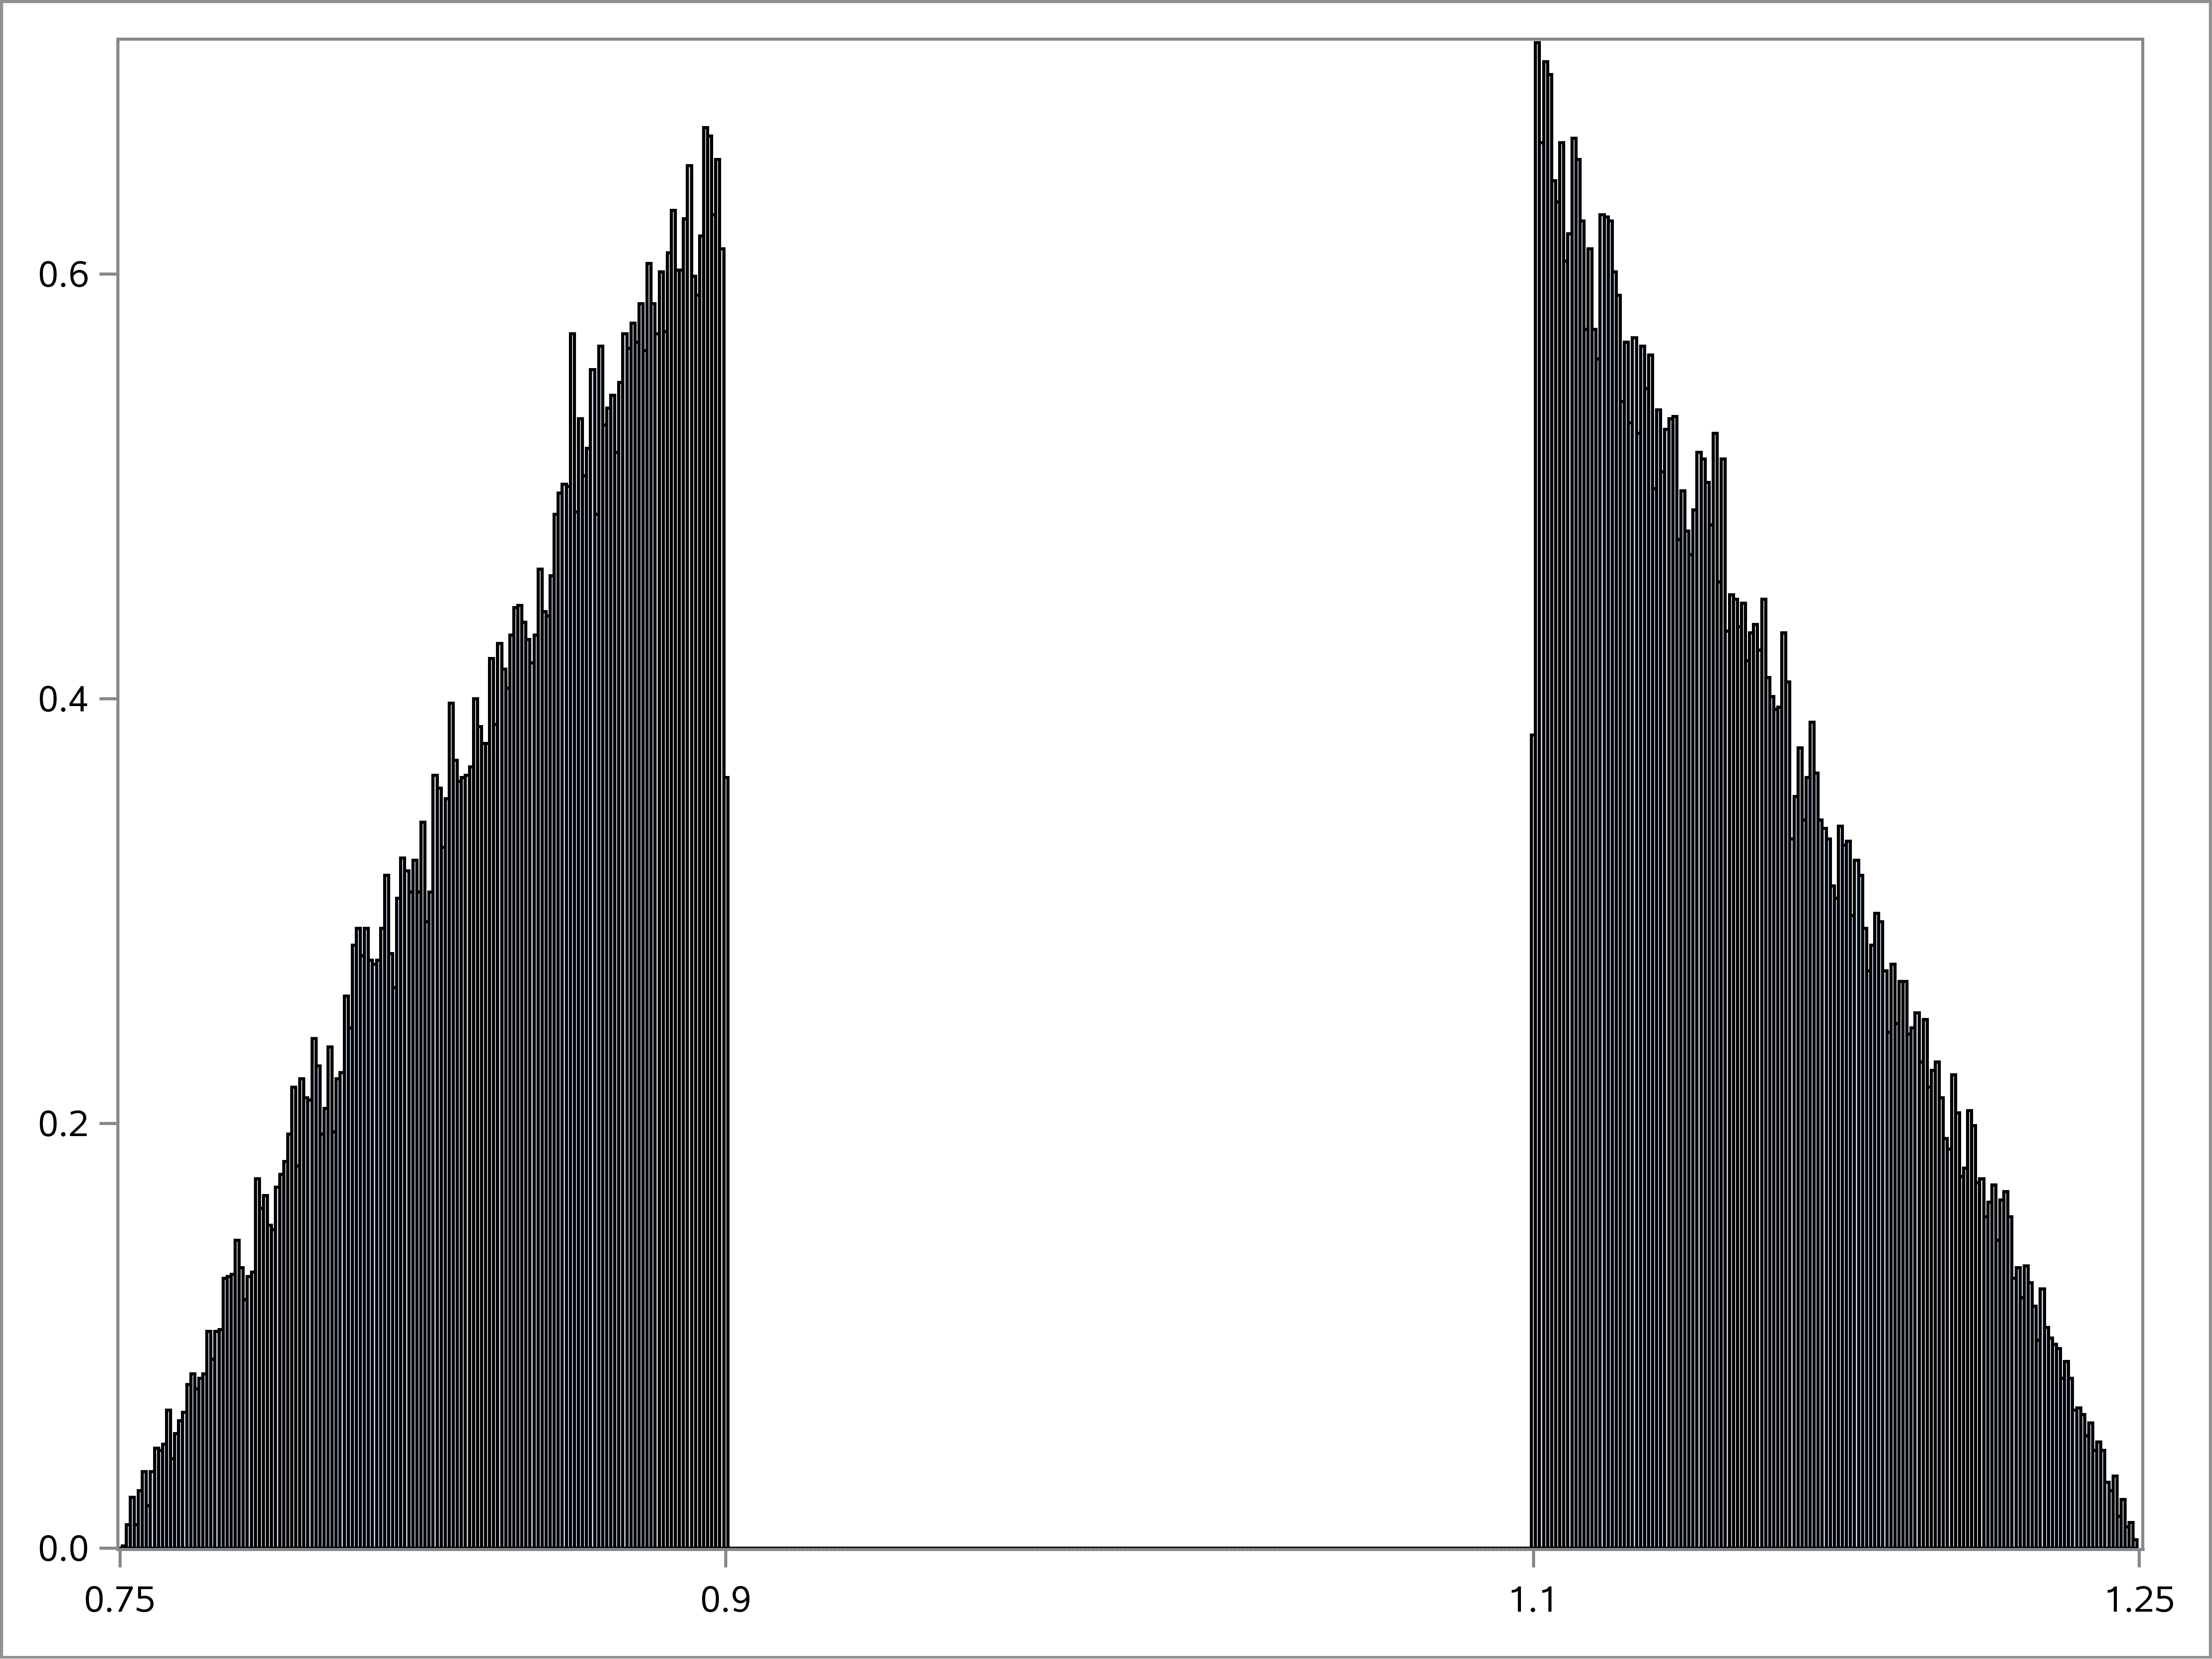
\includegraphics[width=0.9\textwidth]{SGPlotHiDef.png}
\end{figure}

\clearpage
\begin{figure}[p]
	\centering
	\caption{Levels of released and synthetic data\label{fig:level_denom}}
	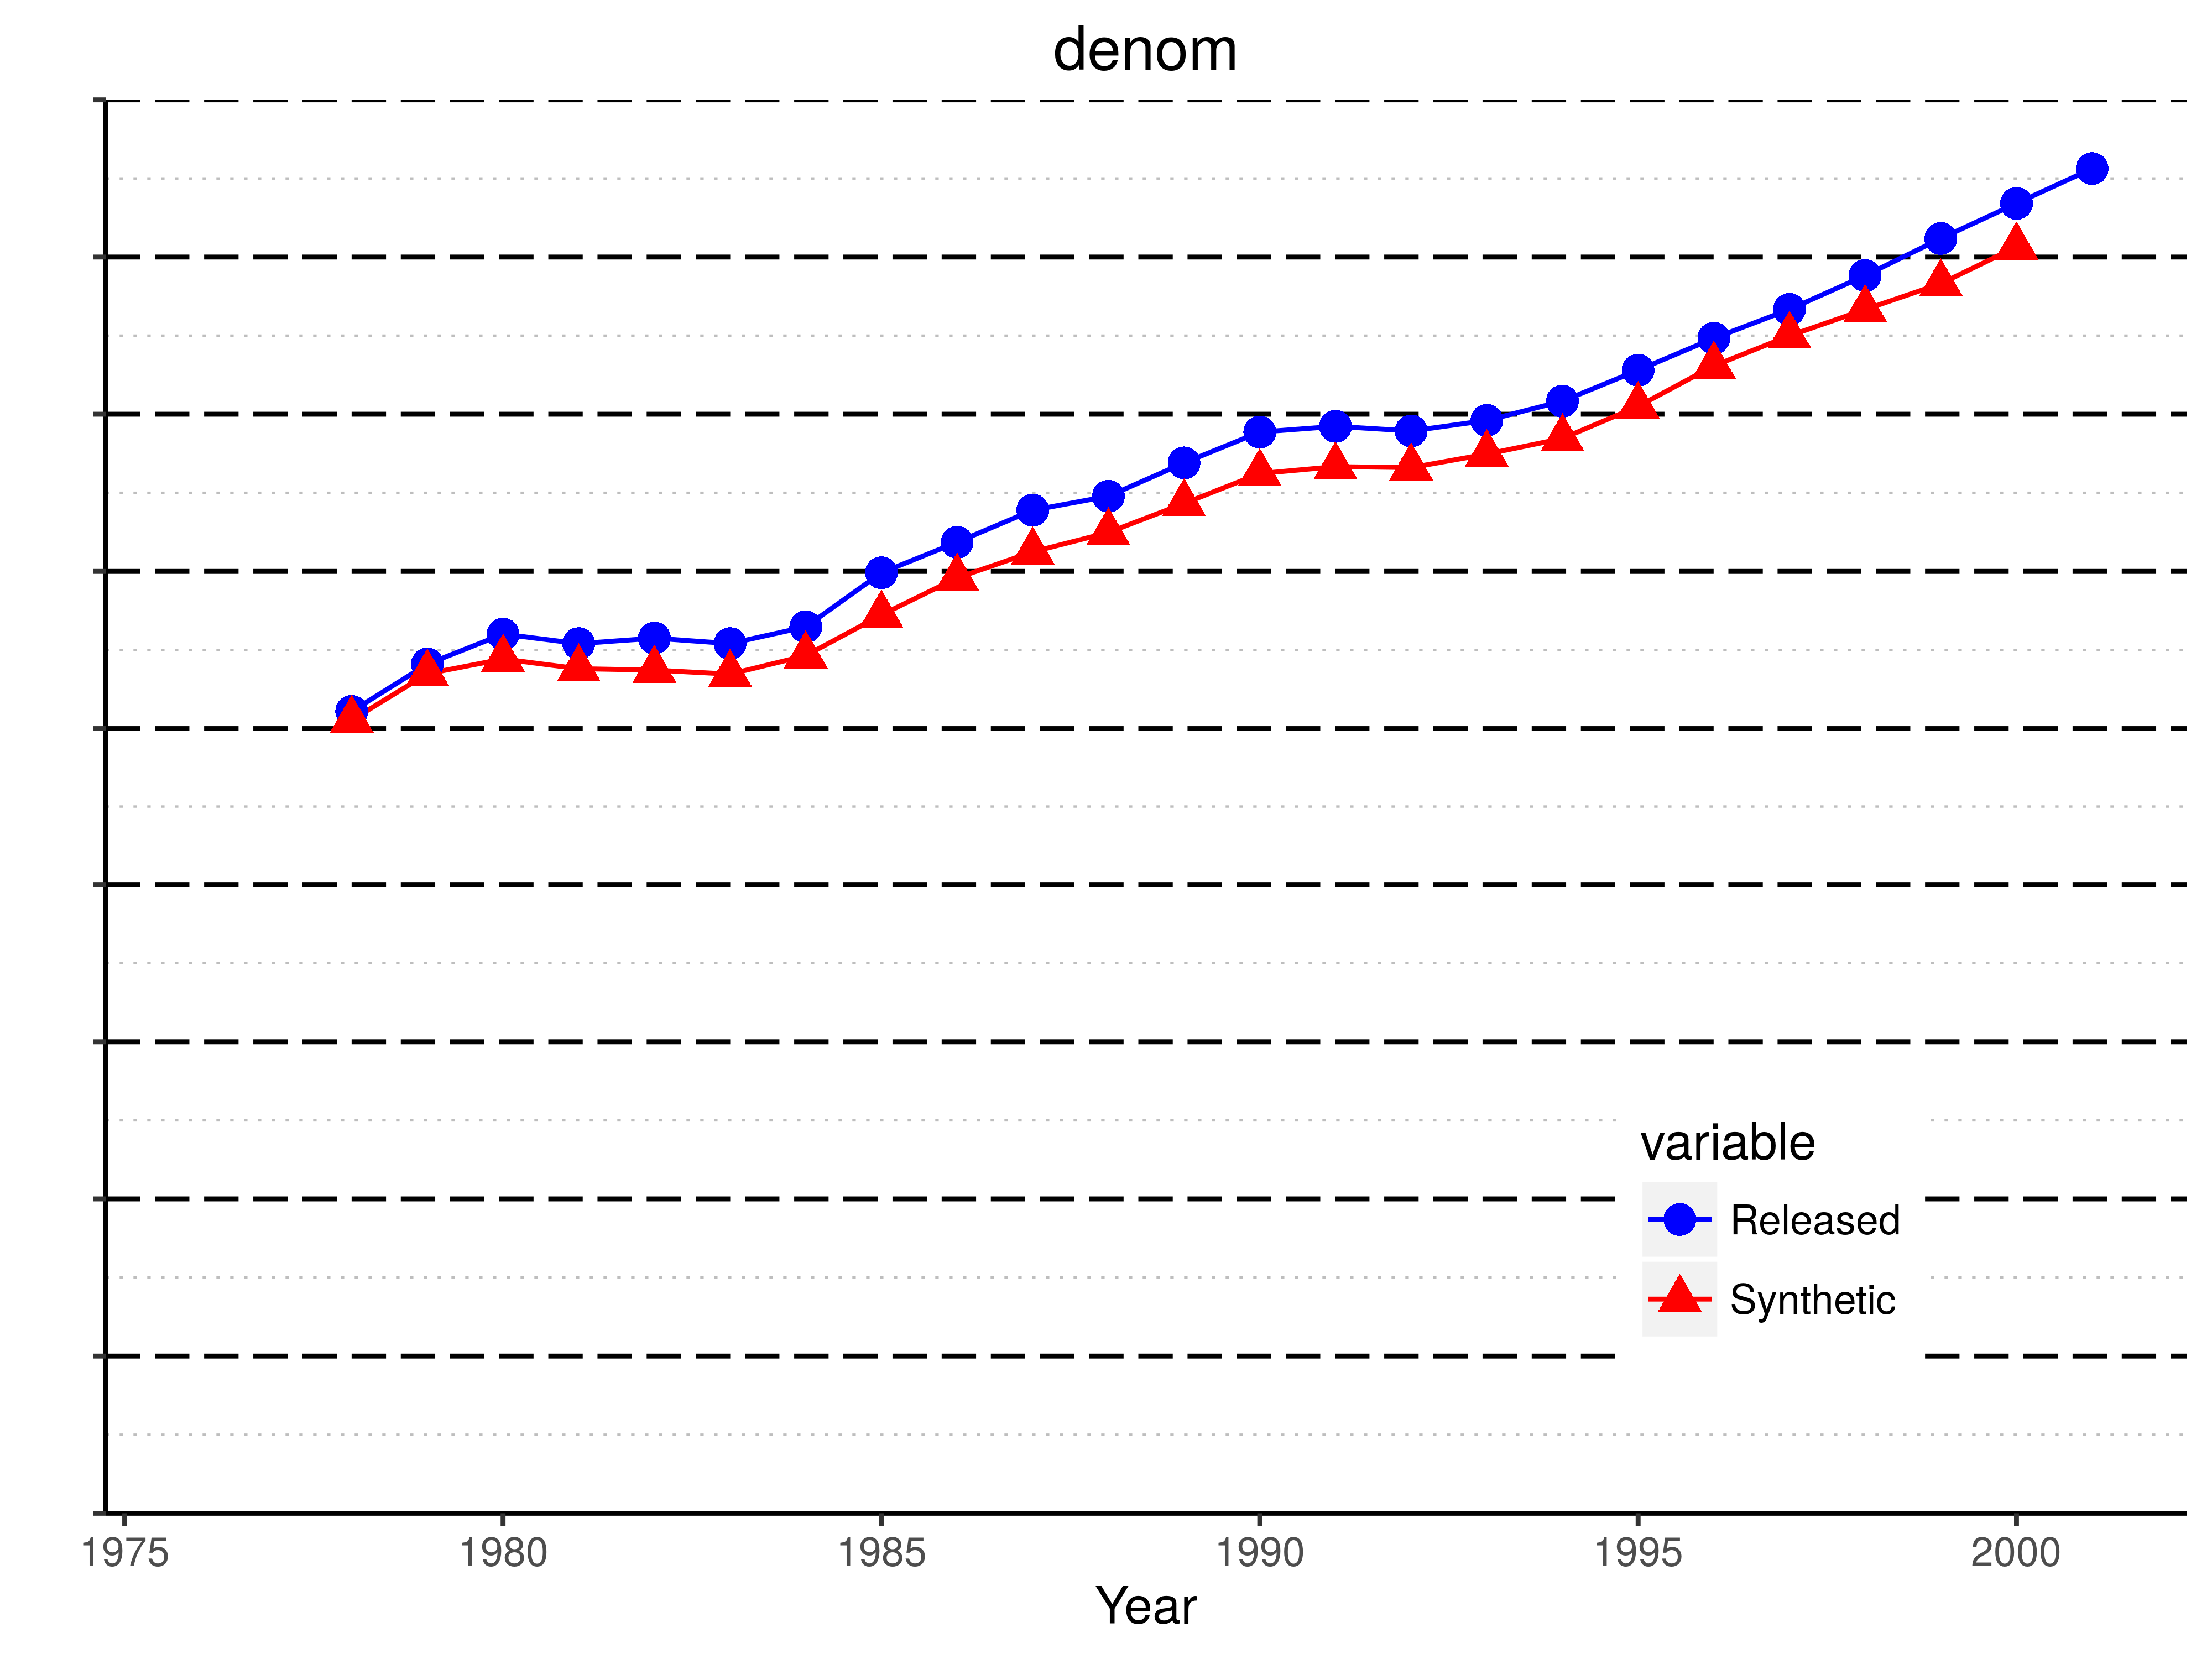
\includegraphics[width=0.45\textwidth]{results/graph_bds_real_vs_syn_denom_R}
	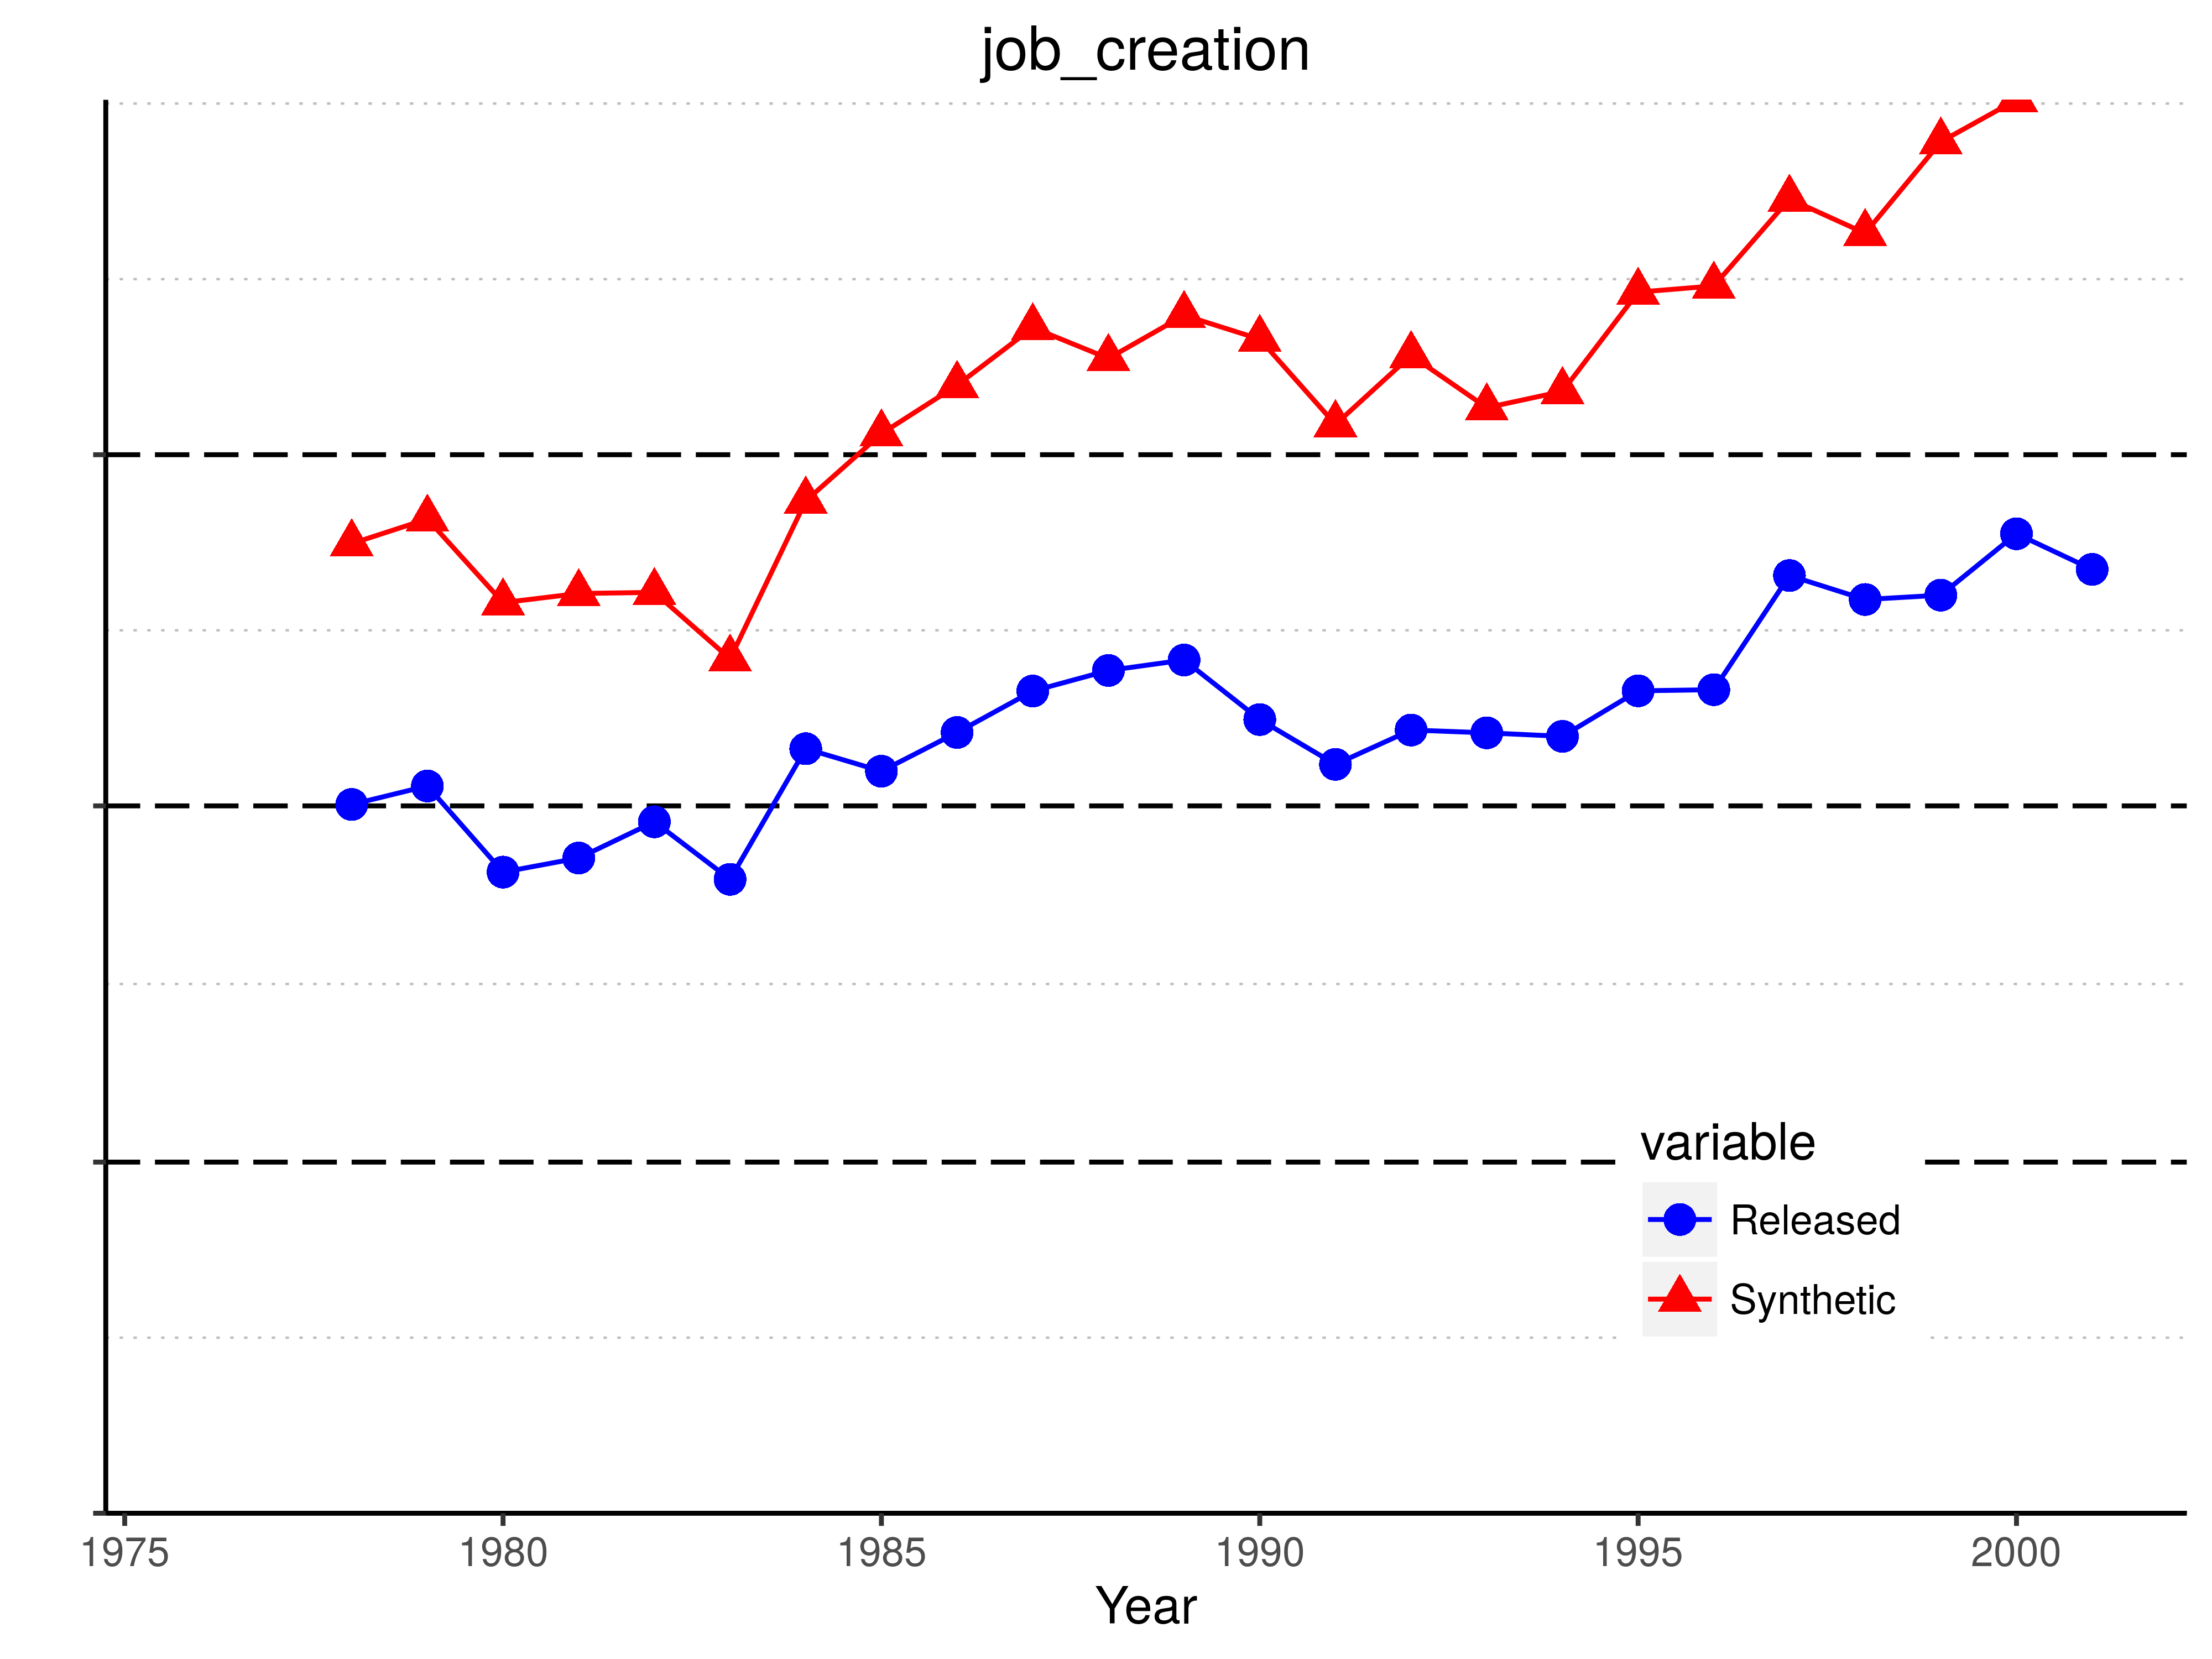
\includegraphics[width=0.45\textwidth]{results/graph_bds_real_vs_syn_job_creation_R}
	
	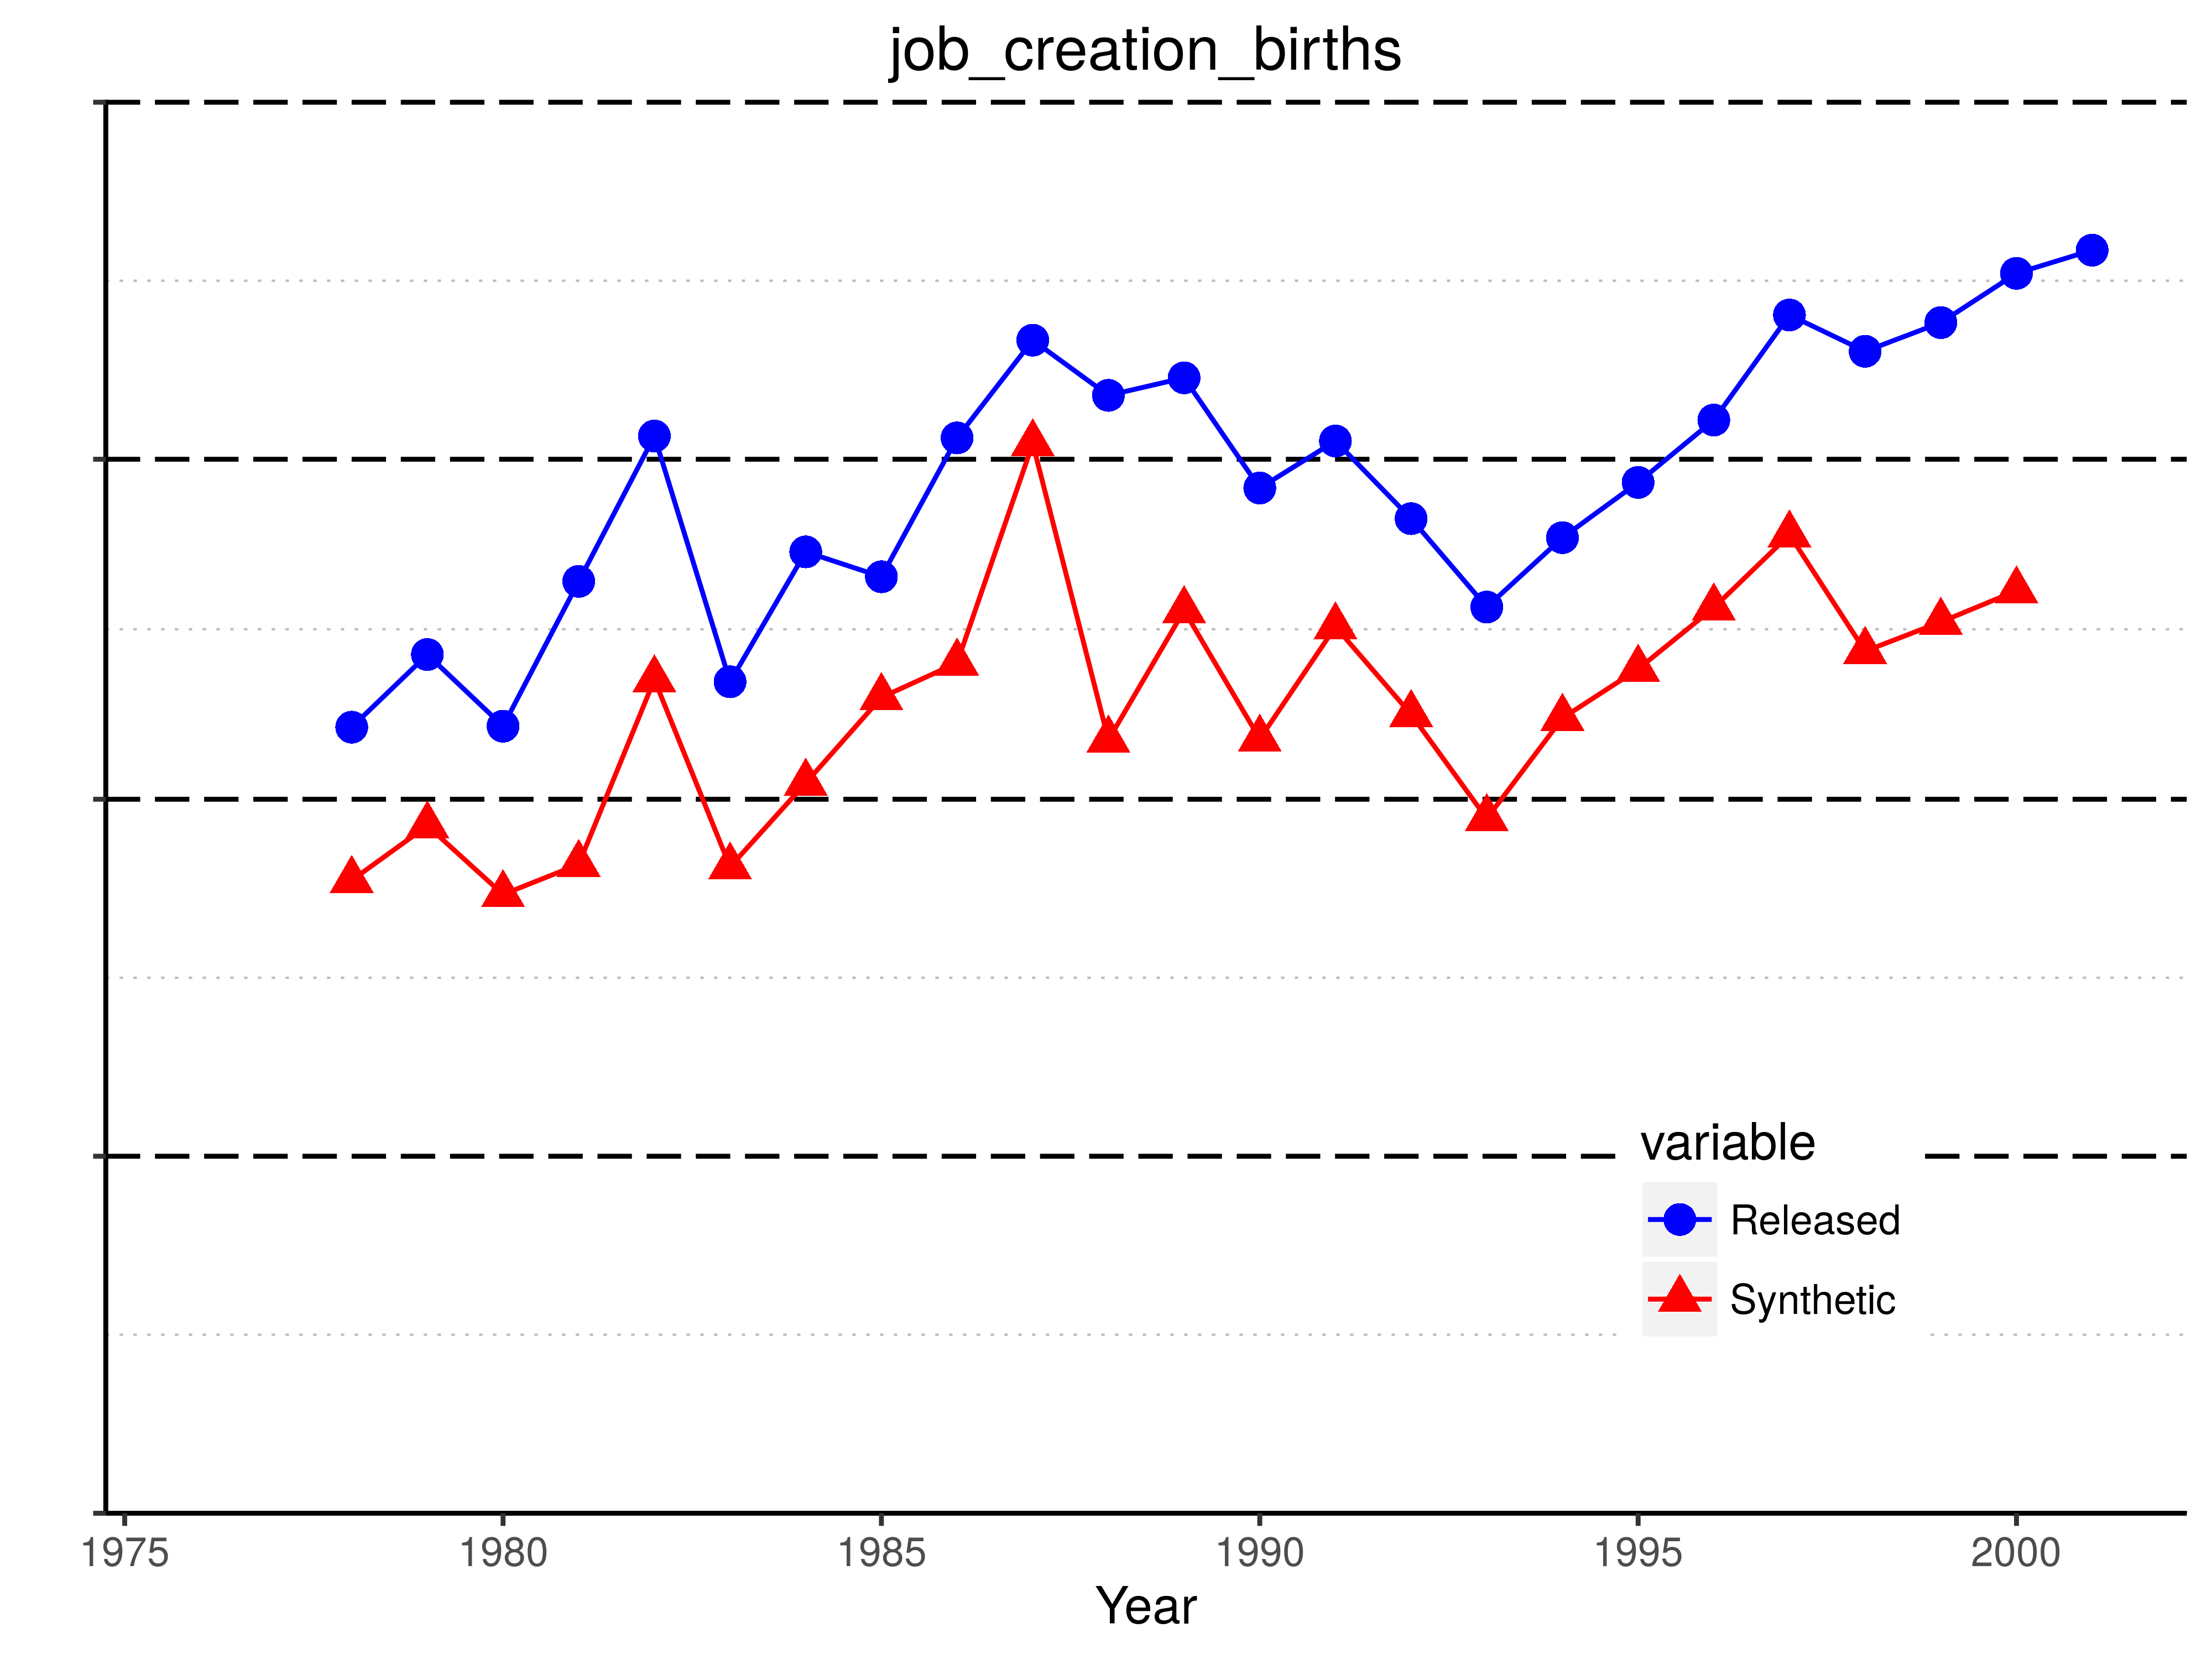
\includegraphics[width=0.45\textwidth]{results/graph_bds_real_vs_syn_job_creation_births_R}
	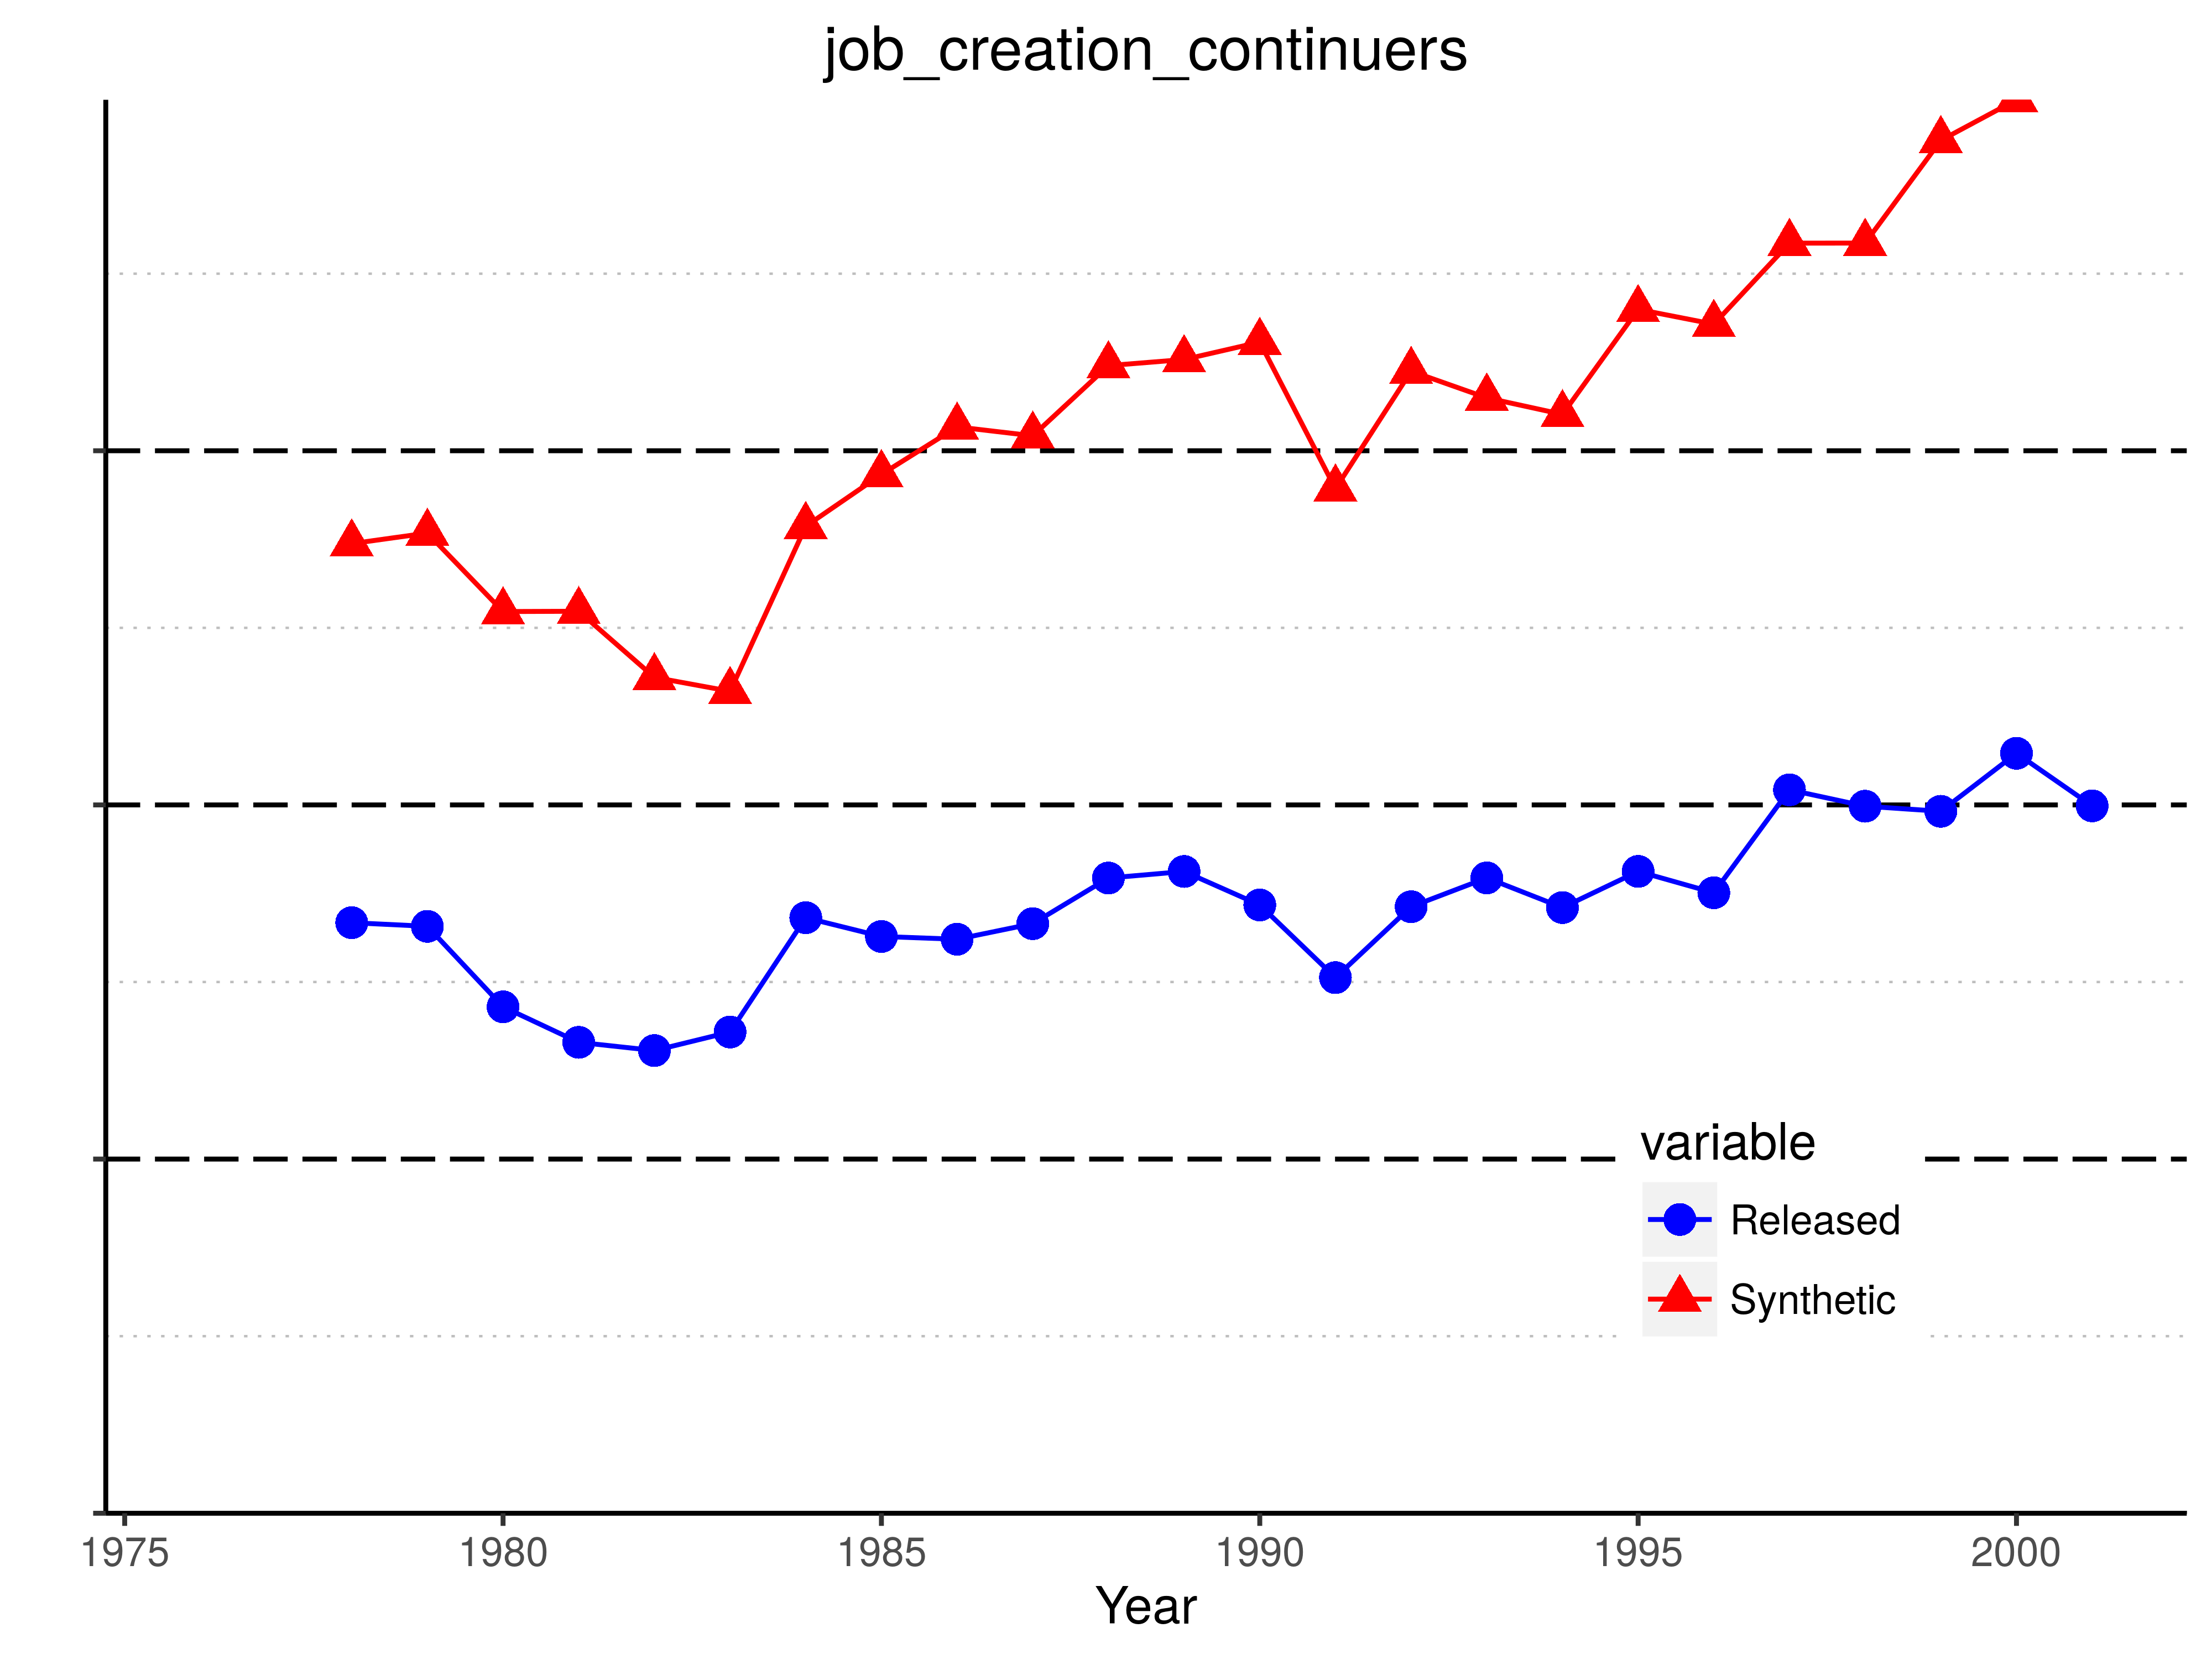
\includegraphics[width=0.45\textwidth]{results/graph_bds_real_vs_syn_job_creation_continuers_R}
\end{figure}

\clearpage
\begin{figure}[p]
\centering
\caption{Differences between released and synthetic data\label{fig:pct_denom}\label{fig:pct_jc}}
%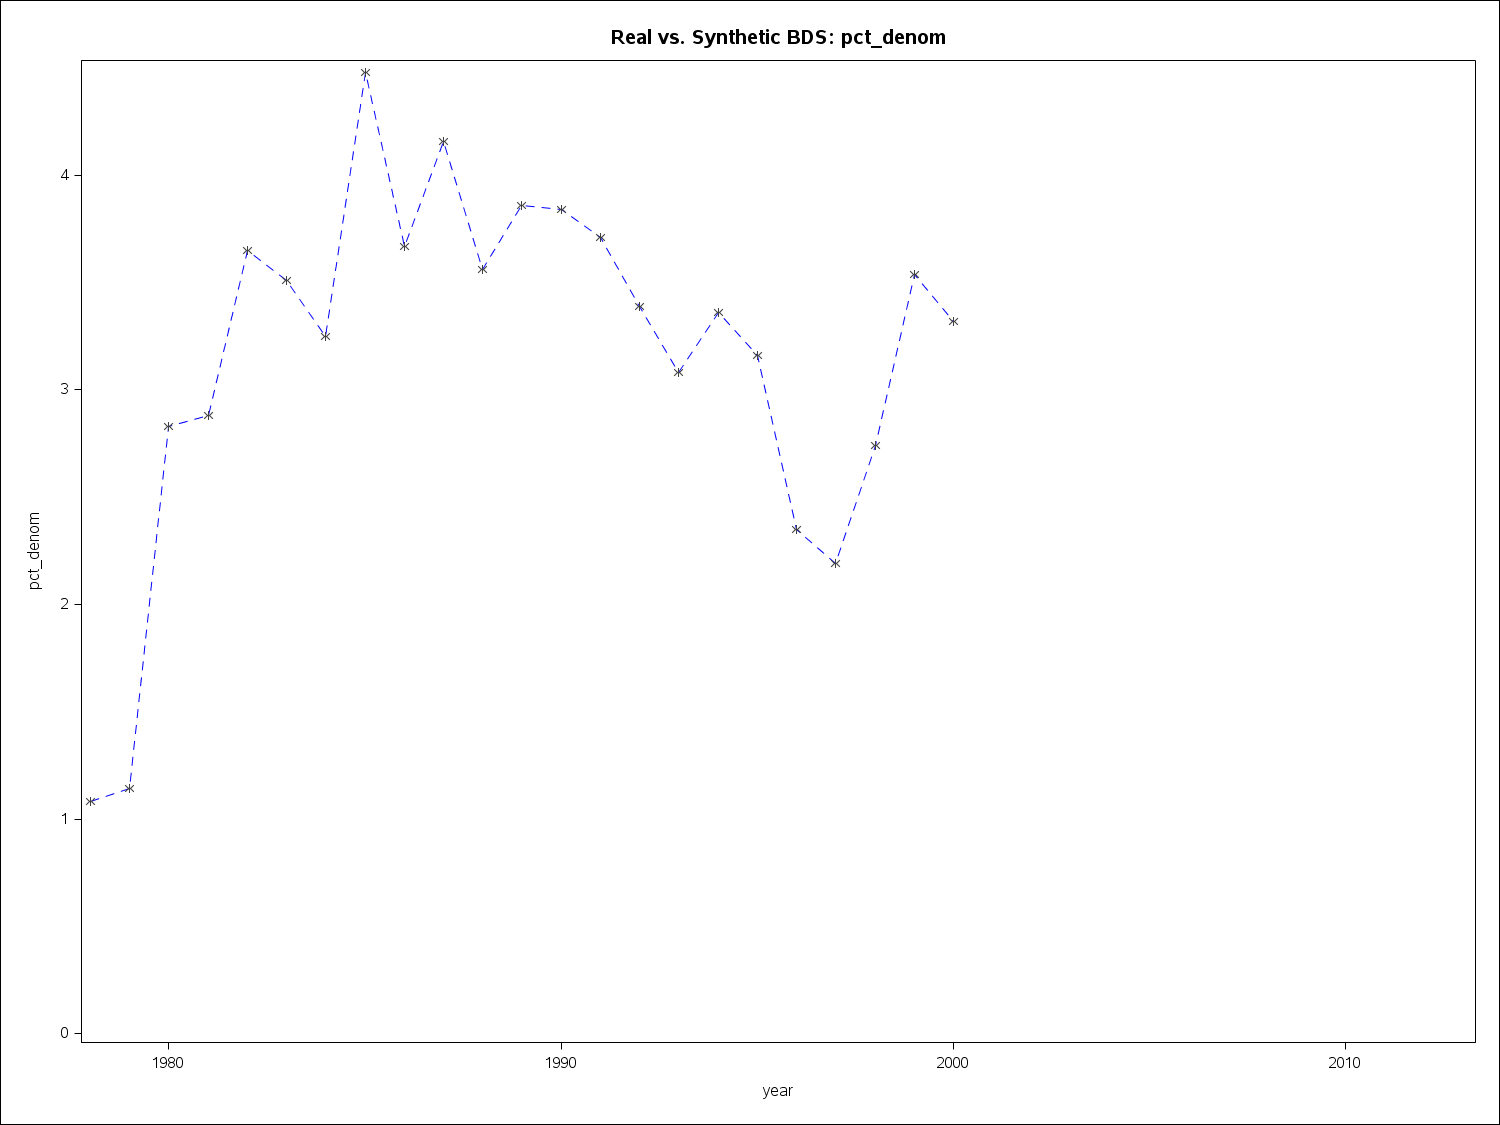
\includegraphics[width=0.45\textwidth]{results/graph_bds_real_vs_syn_pct_denom}
%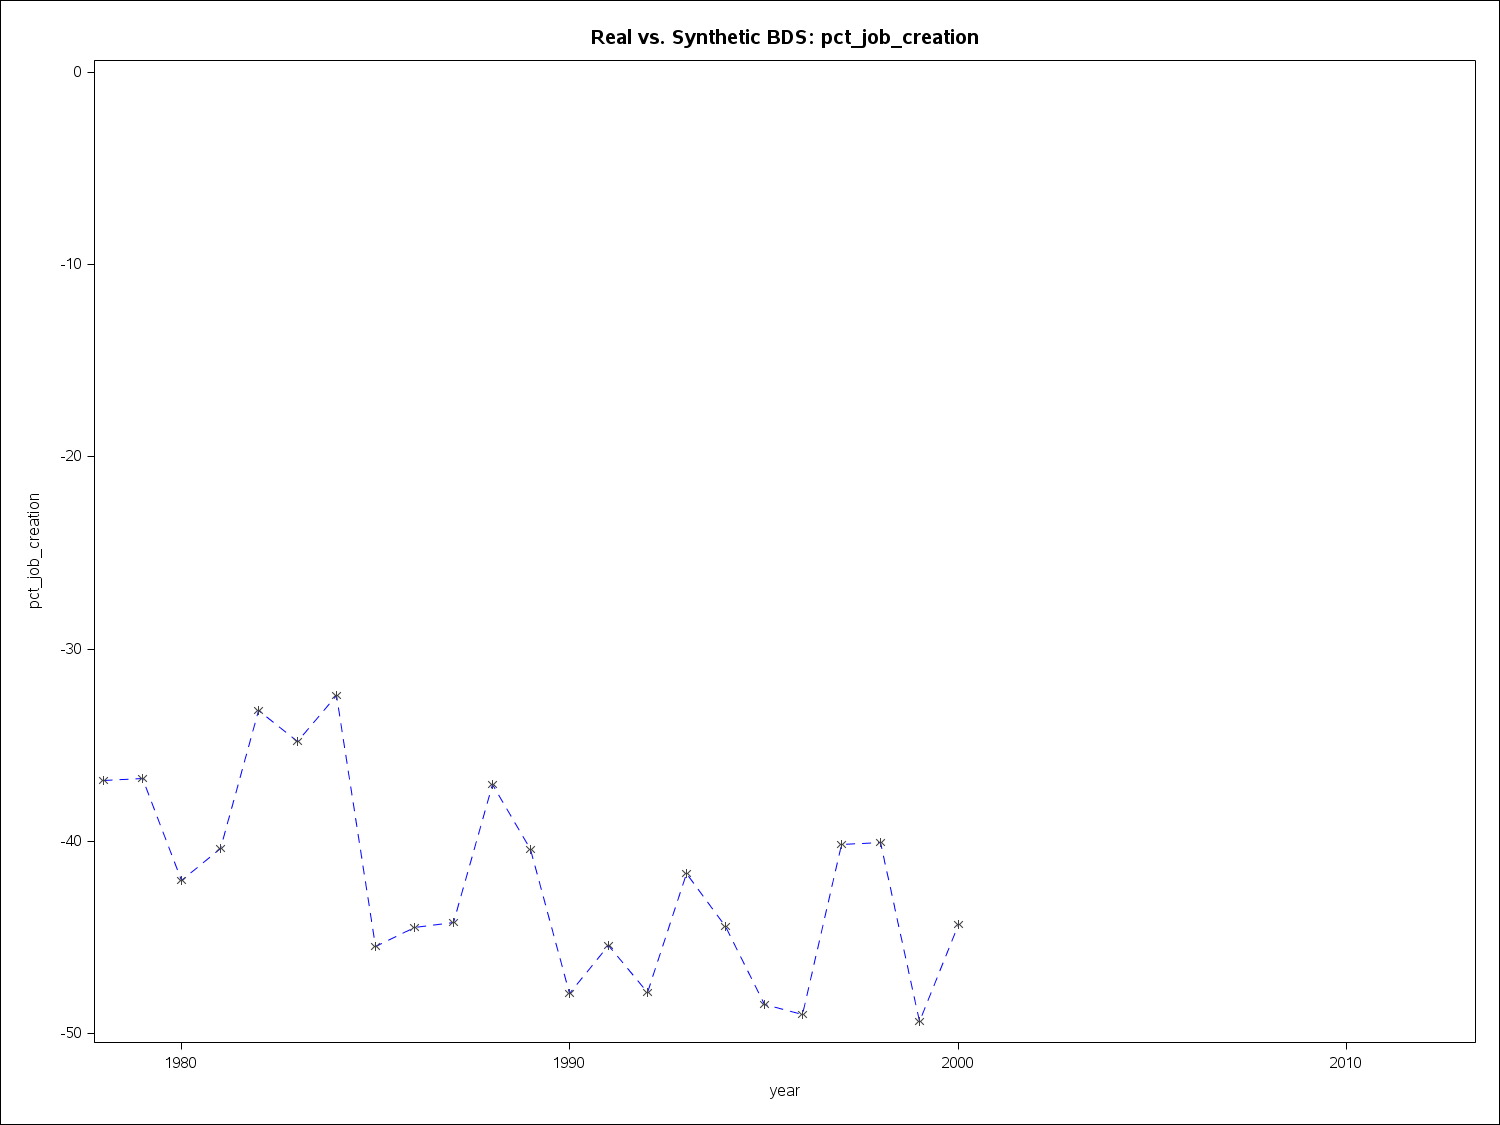
\includegraphics[width=0.45\textwidth]{results/graph_bds_real_vs_syn_pct_job_creation}
%
%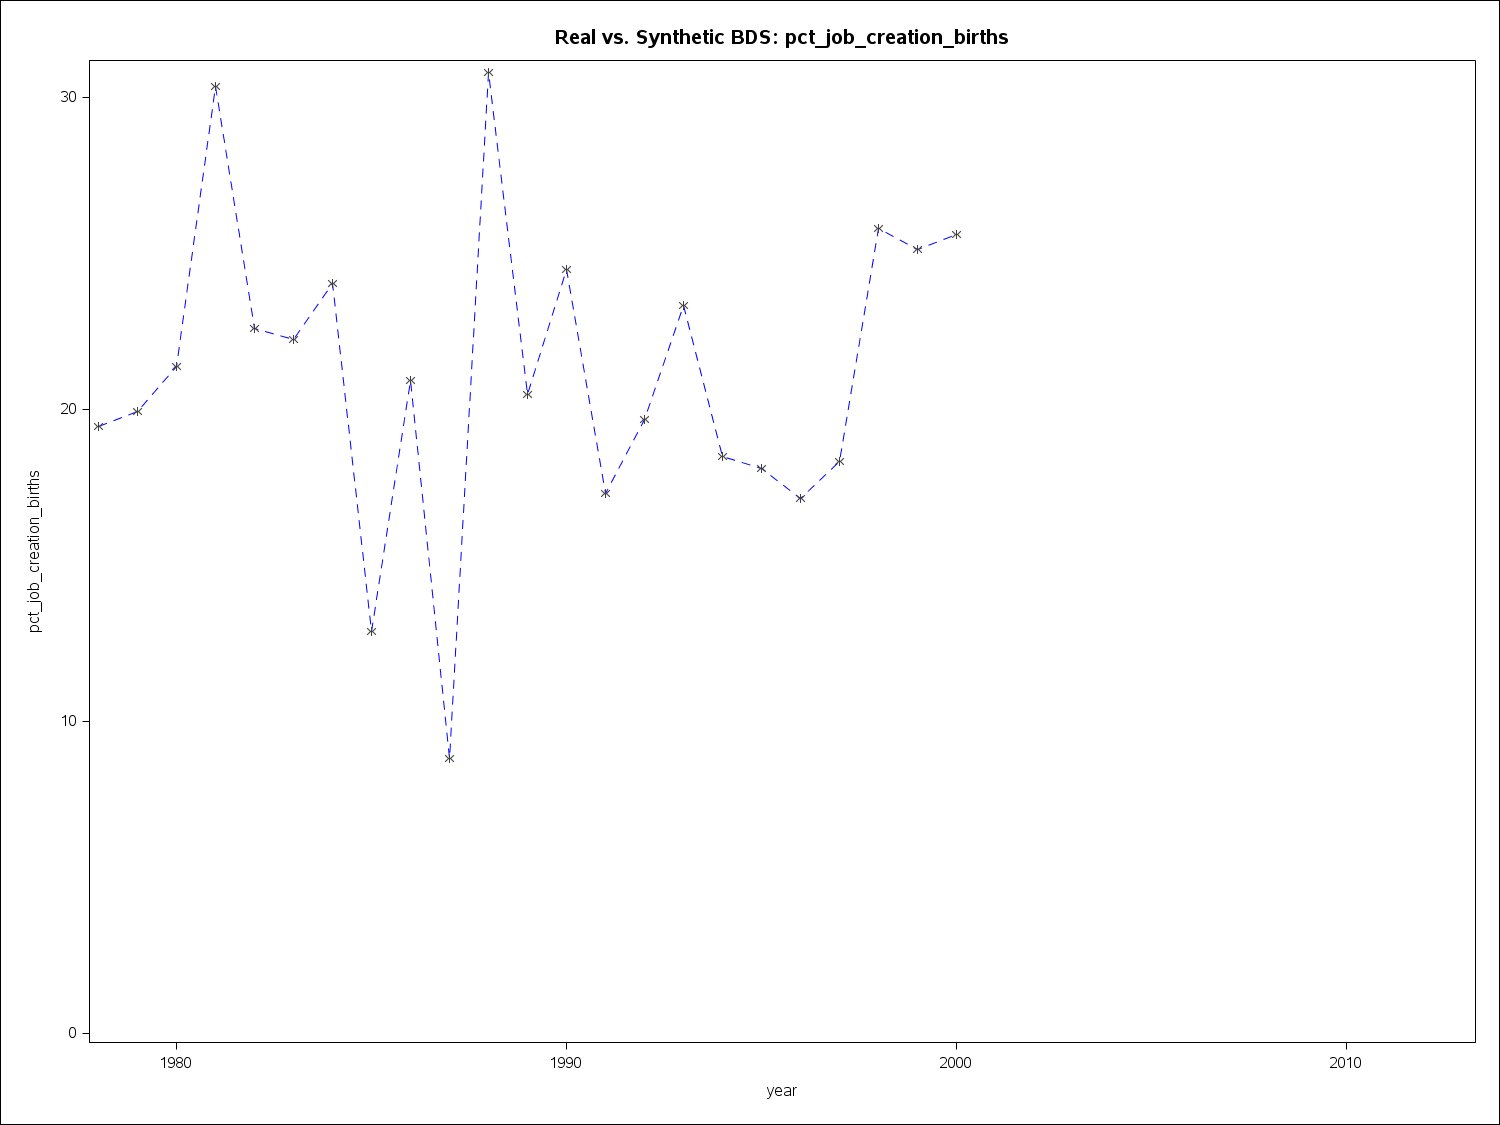
\includegraphics[width=0.45\textwidth]{results/graph_bds_real_vs_syn_pct_job_creation_births}
%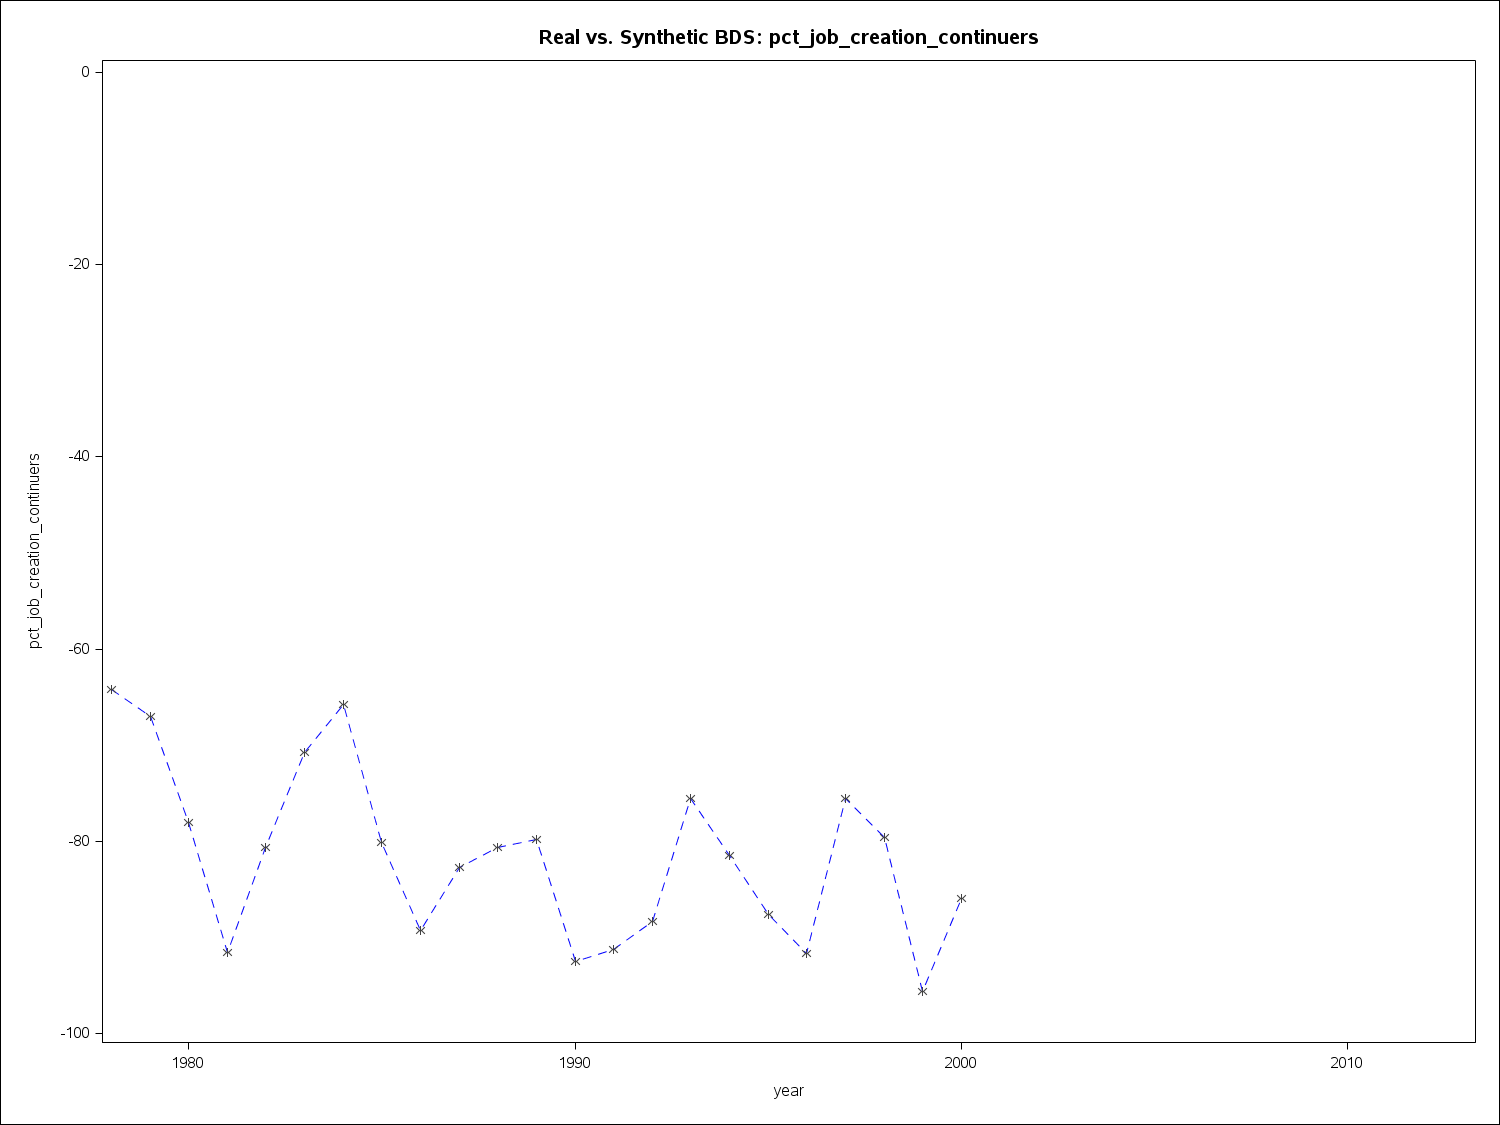
\includegraphics[width=0.45\textwidth]{results/graph_bds_real_vs_syn_pct_job_creation_continuers}
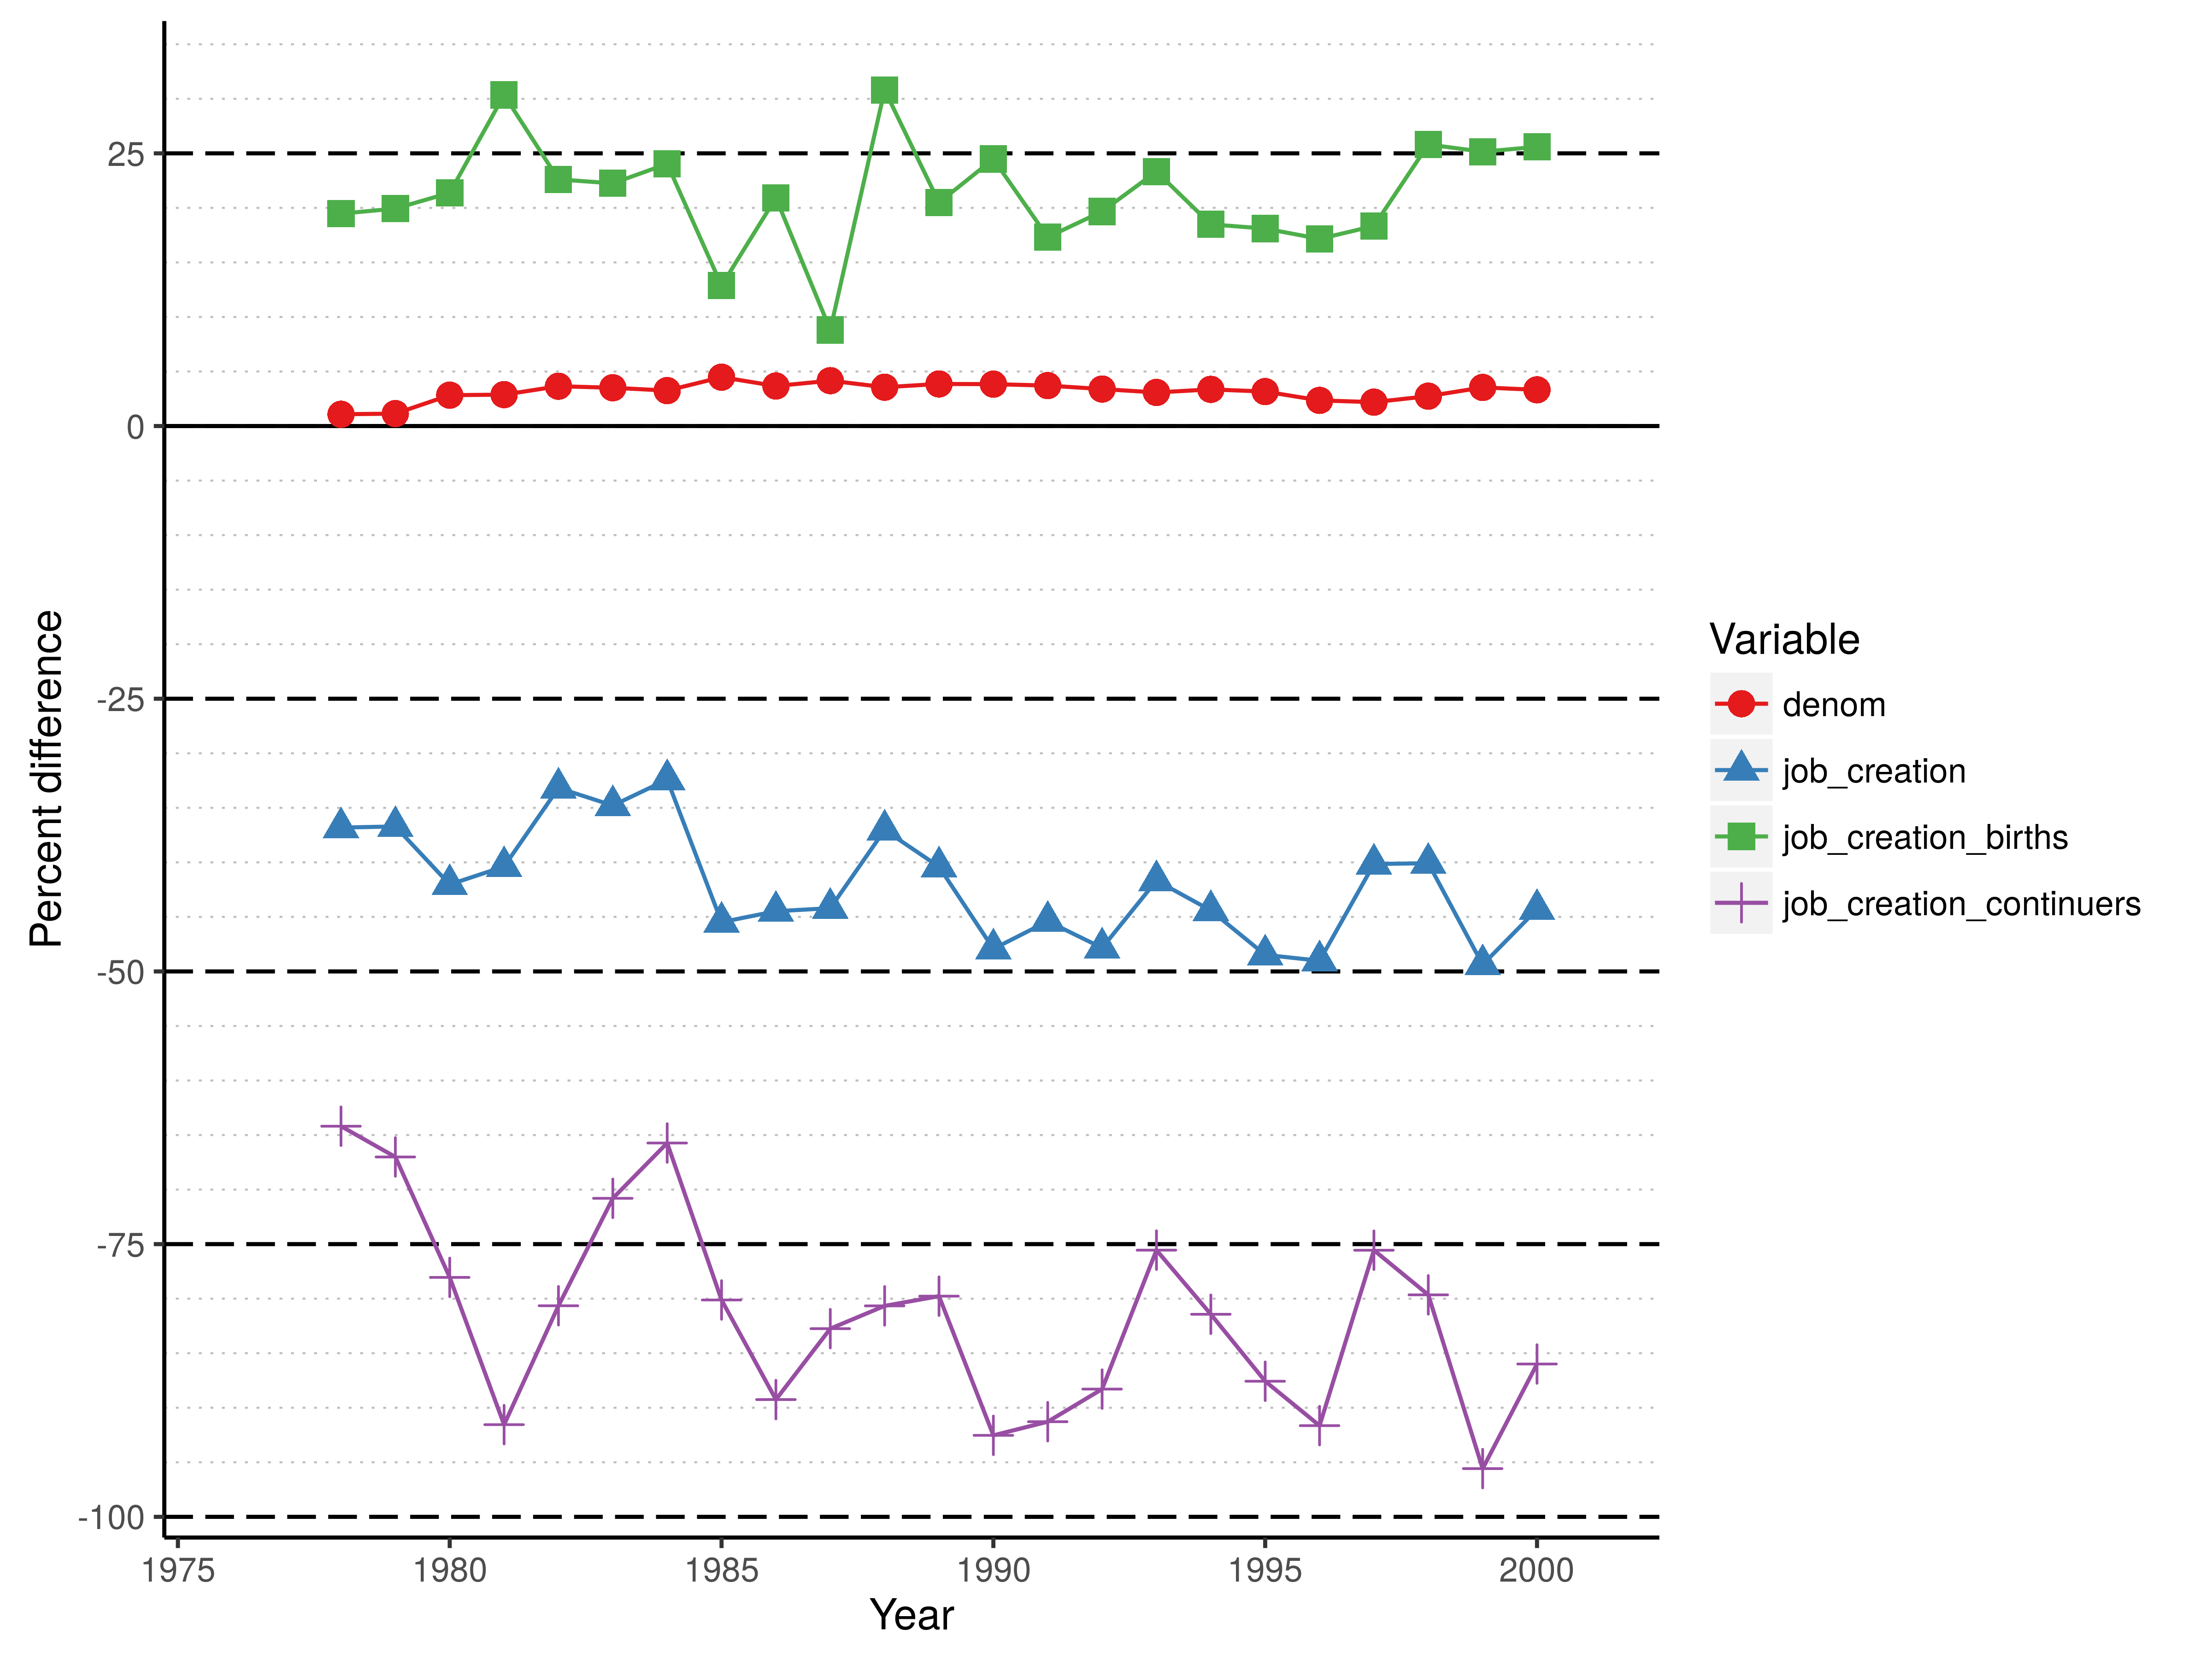
\includegraphics[width=\textwidth]{results/pct_diff_8in}
\end{figure}



\clearpage
{\tiny
\begin{verbatim}
        This version: $Id: synbds-noise-synthetic-SJIAOS2015.tex 1784 2016-01-06 14:56:56Z lv39 $
\end{verbatim}
}
\end{document}
